\chapter{Evaluation}
\label{chap:evaluation}
This chapter covers the quantitative and qualitative evaluation of all four models (LNN, TCN, LSTM, and Transformer) on the same input under various adversarial conditions. We systematically assess how each architecture responds to different types of perturbations, focusing on both performance degradation and qualitative failure modes. These metrics are chosen to capture both the accuracy of trajectory predictions and the model's stability and response to input changes.

\section{Evaluation Metrics}

\subsubsection*{1. Mean Squared Error (MSE)}
The loss function used during training was the Mean Squared Error, given by:
\[
\text{MSE} = \frac{1}{T} \sum_{t=1}^{T} \| \hat{x}_t - x_t \|_2^2
\]
where $\hat{x}_t$ is the predicted output at time $t$, and $x_t$ is the ground truth. MSE measures the average difference between predicted and true trajectories, and is used as a baseline measure of performance under clean (non-adversarial) conditions.

\subsubsection*{2. Degradation Ratio}
To evaluate adversarial impact, the degradation ratio is defined as:
\[
\text{Degradation} = \frac{\text{MSE}_{\text{adv}} - \text{MSE}_{\text{clean}}}{\text{MSE}_{\text{clean}} + \delta}
\]
where $\delta$ is a small constant added to avoid division by zero. This metric captures the relative performance decrease caused by adversarial perturbations. This helps to compare vulnerability across models regardless of their baseline MSE.

\subsubsection*{3. Deviation Distance}
The $\ell_2$ deviation between the clean and adversarial predictions is calculated as:
\[
\text{Deviation} = \frac{1}{T} \sum_{t=1}^{T} \| \hat{x}_t^{\text{adv}} - \hat{x}_t^{\text{clean}} \|_2
\]
This metric quantifies the visible divergence in predicted trajectories.

Unlike degradation ratio, which depends on the ground truth, this metric focuses purely on how much the model's output changes under perturbation. It is a task-independent measure of functional instability, showing how sensitive the model's outputs are to small adversarial changes.

\subsubsection*{4. Local Sensitivity (Lipschitz Estimate)}
To characterise the smoothness of the model's function, local sensitivity is estimated by:
\[
\text{Sensitivity} = \frac{\| \hat{x}^{\text{adv}} - \hat{x}^{\text{clean}} \|_2}{\| x^{\text{adv}} - x^{\text{clean}} \|_2}
\]
This ratio approximates the local Lipschitz constant, capturing how much the output changes in response to small input perturbations. A higher sensitivity indicates that the model has sharp local gradients, potentially making it more brittle. This provides a theoretical metric for robustness, independent of task-specific loss.

\section{Quantitative Results}

\subsection*{Aggregate Metrics Across All Attacks}

\begin{table}[H]
    \centering
    \begin{tabular}{|l|c|c|c|c|}
    \hline
    \textbf{Model} & \textbf{Avg. Degradation \%} & \textbf{Avg. Deviation} & \textbf{Avg. Lipschitz Estimate} & \textbf{Clean MSE} \\
    \hline
    LNN         & 417.8377 & 2.1646 & 0.9441 & 0.0028 \\
    TCN         & 434.2948 & 2.2409 & 1.0071 & 0.0028 \\
    LSTM        & 287.4266 & 2.1501 & 1.0132 & 0.0044 \\
    Transformer & 183.5425 & 2.3060 & 1.1352 & 0.0077 \\
    \hline
    \end{tabular}
    \caption{Average robustness metrics across all attacks. Lower values are better for all columns.}
    \label{tab:avg_model_robustness}
\end{table}

Importantly, each model was designed/trained to have comparable MSEs, to allow for fair evaluation.

\begin{figure}[H]
    \centering
    
    \begin{subfigure}[t]{0.45\linewidth}
    \centering
    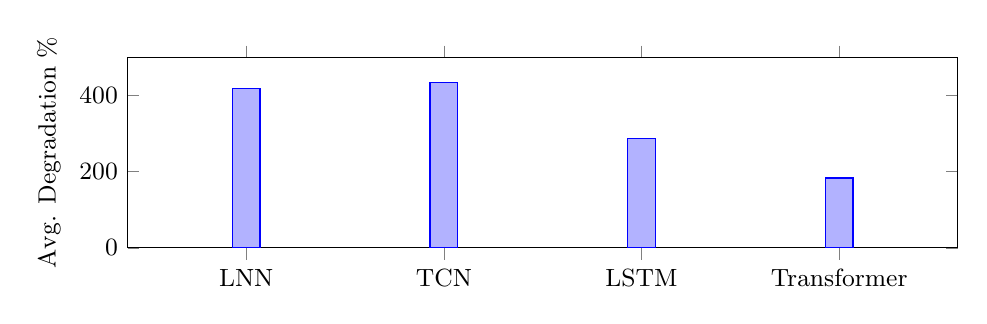
\begin{tikzpicture}
    \begin{axis}[
        ybar,
        ylabel={Avg. Degradation \%},
        xtick=data,
        xticklabels={LNN, TCN, LSTM, Transformer},
        ymin=0, ymax=500,
        bar width=10pt,
        width=\linewidth,
        height=4cm,
        enlarge x limits=0.2,
        ylabel style={font=\small},
        tick label style={font=\small}
    ]
    \addplot coordinates {(0,417.8377) (1,434.2948) (2,287.4266) (3,183.5425)};
    \end{axis}
    \end{tikzpicture}
    \caption{Average Degradation}
    \end{subfigure}
    \hfill
    \begin{subfigure}[t]{0.45\linewidth}
    \centering
    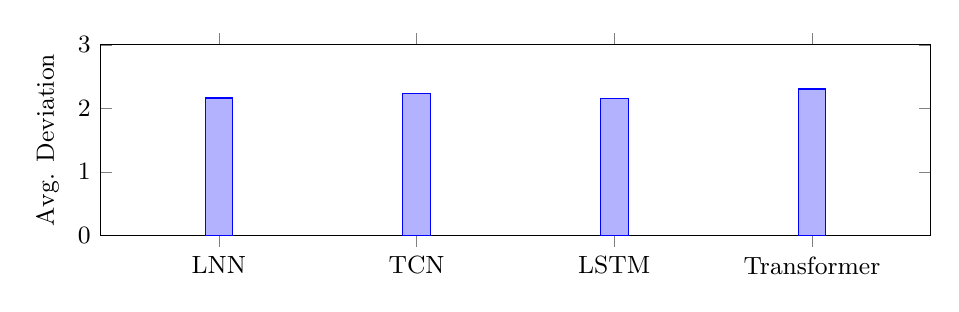
\begin{tikzpicture}
    \begin{axis}[
        ybar,
        ylabel={Avg. Deviation},
        xtick=data,
        xticklabels={LNN, TCN, LSTM, Transformer},
        ymin=0, ymax=3,
        bar width=10pt,
        width=\linewidth,
        height=4cm,
        enlarge x limits=0.2,
        ylabel style={font=\small},
        tick label style={font=\small}
    ]
    \addplot coordinates {(0,2.1646) (1,2.2409) (2,2.1501) (3,2.3060)};
    \end{axis}
    \end{tikzpicture}
    \caption{Average Deviation}
    \end{subfigure}
    
    \vspace{0.8em}
    
    \begin{subfigure}[t]{0.45\linewidth}
    \centering
    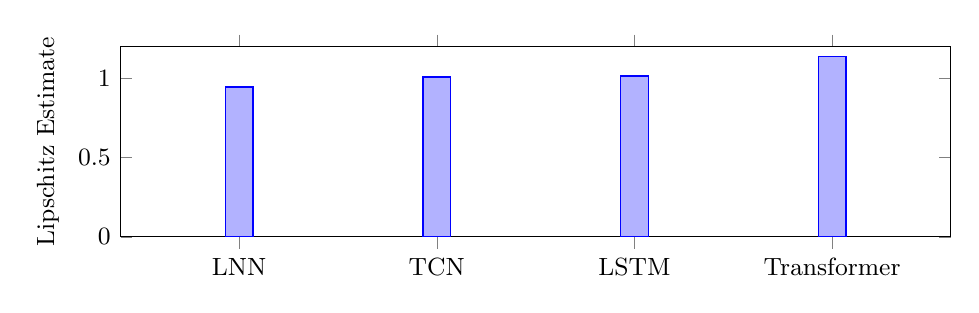
\begin{tikzpicture}
    \begin{axis}[
        ybar,
        ylabel={Lipschitz Estimate},
        xtick=data,
        xticklabels={LNN, TCN, LSTM, Transformer},
        ymin=0, ymax=1.2,
        bar width=10pt,
        width=\linewidth,
        height=4cm,
        enlarge x limits=0.2,
        ylabel style={font=\small},
        tick label style={font=\small}
    ]
    \addplot coordinates {(0,0.9441) (1,1.0071) (2,1.0132) (3,1.1352)};
    \end{axis}
    \end{tikzpicture}
    \caption{Lipschitz Estimate}
    \end{subfigure}
    \hfill
    \begin{subfigure}[t]{0.45\linewidth}
    \centering
    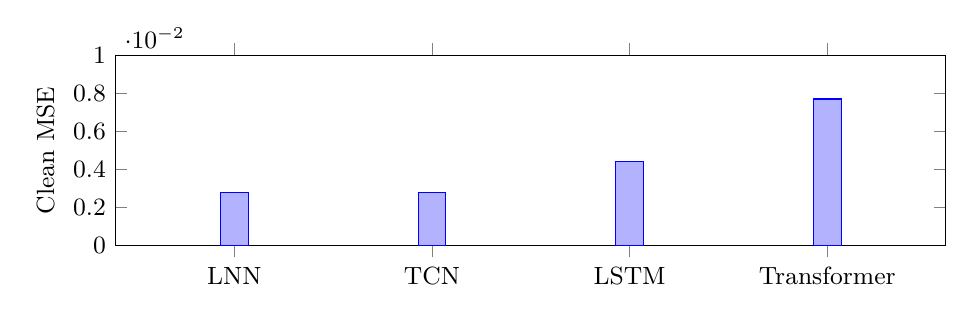
\begin{tikzpicture}
    \begin{axis}[
        ybar,
        ylabel={Clean MSE},
        xtick=data,
        xticklabels={LNN, TCN, LSTM, Transformer},
        ymin=0, ymax=0.01,
        bar width=10pt,
        width=\linewidth,
        height=4cm,
        enlarge x limits=0.2,
        ylabel style={font=\small},
        tick label style={font=\small}
    ]
    \addplot coordinates {(0,0.0028) (1,0.0028) (2,0.0044) (3,0.0077)};
    \end{axis}
    \end{tikzpicture}
    \caption{Clean MSE}
    \end{subfigure}
    
    \caption{Average robustness metrics by model across all attacks. Lower is better.}
    \label{fig:avg_metrics_barplot}
    \end{figure}

\subsection*{Attack-Specific Results}

The following tables summarise each metric for each model, under various adversarial attacks. Lower values, across all metrics, indicate better robustness.

\begin{table}[H]
    \centering
    \small
    \begin{tabular}{|l|cccc|}
    \hline
    \textbf{Attack Type} & \multicolumn{4}{c|}{\textbf{Degradation (\%)}} \\
    \cline{2-5}
     & \textbf{LNN} & \textbf{TCN} & \textbf{LSTM} & \textbf{Transformer} \\
    \hline
    FGSM                     & 209.6842 & 242.5555 & 169.5259 & 122.8652 \\
    PGD                      & 209.6700 & 241.7085 & 169.5408 & 127.9633 \\
    DeepFool-inspired        & 12.5395 & 13.9643 & 11.2735 & 8.8294 \\
    SPSA                     & 36.8717 & 47.0328 & 29.7149 & 21.6053 \\
    Time-Warping             & 1576.5198 & 1664.5960 & 1033.6341 & 579.3263 \\
    Continuous-Time Perturb. & 458.7058 & 435.9864 & 329.8787 & 242.7071 \\
    \hline
    \end{tabular}
    \caption{Degradation ratios across models for each attack}
    \label{tab:attack_results_degradation}
\end{table}

\begin{table}[H]
    \centering
    \small
    \begin{tabular}{|l|cccc|}
    \hline
    \textbf{Attack Type} & \multicolumn{4}{c|}{\textbf{Deviation}} \\
    \cline{2-5}
     & \textbf{LNN} & \textbf{TCN} & \textbf{LSTM} & \textbf{Transformer} \\
    \hline
    FGSM                     & 1.293169 & 1.419442 & 1.367006 & 1.474218 \\
    PGD                      & 1.293832 & 1.416078 & 1.367387 & 1.527660 \\
    DeepFool-inspired        & 0.096296 & 0.101111 & 0.111709 & 0.148173 \\
    SPSA                     & 0.777944 & 0.876160 & 0.842481 & 0.919706 \\
    Time-Warping             & 6.953865 & 7.026645 & 6.882243 & 7.036172 \\
    Continuous-Time Perturb. & 2.634408 & 2.599266 & 2.601533 & 2.717356 \\
    \hline
    \end{tabular}
    \caption{Deviation scores across models for each attack}
    \label{tab:attack_results_deviation}
\end{table}

\begin{table}[H]
    \centering
    \small
    \begin{tabular}{|l|cccc|}
    \hline
    \textbf{Attack Type} & \multicolumn{4}{c|}{\textbf{Local Sensitivity (Lipschitz Estimate)}} \\
    \cline{2-5}
     & \textbf{LNN} & \textbf{TCN} & \textbf{LSTM} & \textbf{Transformer} \\
    \hline
    FGSM                     & 0.915554 & 1.004954 & 0.967830 & 1.043735 \\
    PGD                      & 0.919326 & 1.005099 & 0.968100 & 1.090577 \\
    DeepFool-inspired        & 0.962984 & 1.011127 & 1.117503 & 1.497606 \\
    SPSA                     & 0.857096 & 1.003862 & 0.964692 & 1.026772 \\
    Time-Warping             & 0.999767 & 1.010231 & 0.989470 & 1.011601 \\
    Continuous-Time Perturb. & 1.011938 & 1.006981 & 1.005773 & 1.053375 \\
    \hline
    \end{tabular}
    \caption{Lipschitz Estimate (local sensitivity) across models for each attack}
    \label{tab:attack_results_sensitivity}
\end{table}

The summary statistics in Table~\ref{tab:avg_model_robustness} and the corresponding bar plots highlight a clear trade-off between clean accuracy and robustness. The Transformer achieves the lowest average degradation ($183.54\%$) and deviation ($2.3060$), suggesting superior resistance to adversarial attacks overall. However, it also has the highest clean MSE ($0.0077$) and Lipschitz sensitivity ($1.1352$), indicating instability under small perturbations and noisier baseline performance. In contrast, the LNN achieves stronger clean performance ($0.0028$ MSE) and a lower Lipschitz constant ($0.9441$), but suffers disproportionately under temporal or continuous-time attacks, inflating its degradation average ($417.84\%$). The TCN, while numerically similar to the LNN, is slightly less stable overall, whereas the LSTM maintains balance, with moderate robustness, the lowest average deviation (with the LNN being close), and the second-best clean accuracy. These findings suggest that robustness is not exculsively defined by architectural depth or sequence modelling capability, but instead emerges from the interaction of inductive bias, temporal sensitivity, and perturbation dynamics.

With the lowest average Lipschitz constant (0.9441), the LNN shows the best local sensitivity profile, meaning small changes in input (under $L_p$ norms) cause relatively small changes in output. This is consistent with its ODE-based temporal smoothing.

The LNN is not the most robust across all attacks/metrics, but it is does outperform in specific settings, especially against local gradient-based noise. It's architecture offers benefits for tasks involving temporal continuity, but requires careful consideration when deployed in environments with adversarial dynamics that align with its solver steps or temporal assumptions.

\section{Visual Analysis}

While quantitative metrics provide a summary view of model degradation, they can obscure the qualitative character of errors, such as spiralling divergence, phase drift, or geometric distortion. In this section, we present visual comparisons between clean and adversarial predictions to better understand how each model's internal representation and output trajectory is disrupted.

\subsection*{Visualisation Methodology}

For each attack and model combination, clean and adversarial predictions were overlaid on the same plot.
Ground truth trajectories were shown for reference, and all sequences were denormalised prior to plotting.

Each figure highlights a specific failure mode characteristic to the architecture under consideration.

\subsection*{FGSM Attack Results}

The FGSM attack was applied to all three models under a fixed perturbation budget $\epsilon = 0.05$. 

\begin{figure}[H]
    \centering
    \begin{subfigure}[b]{0.45\linewidth}
        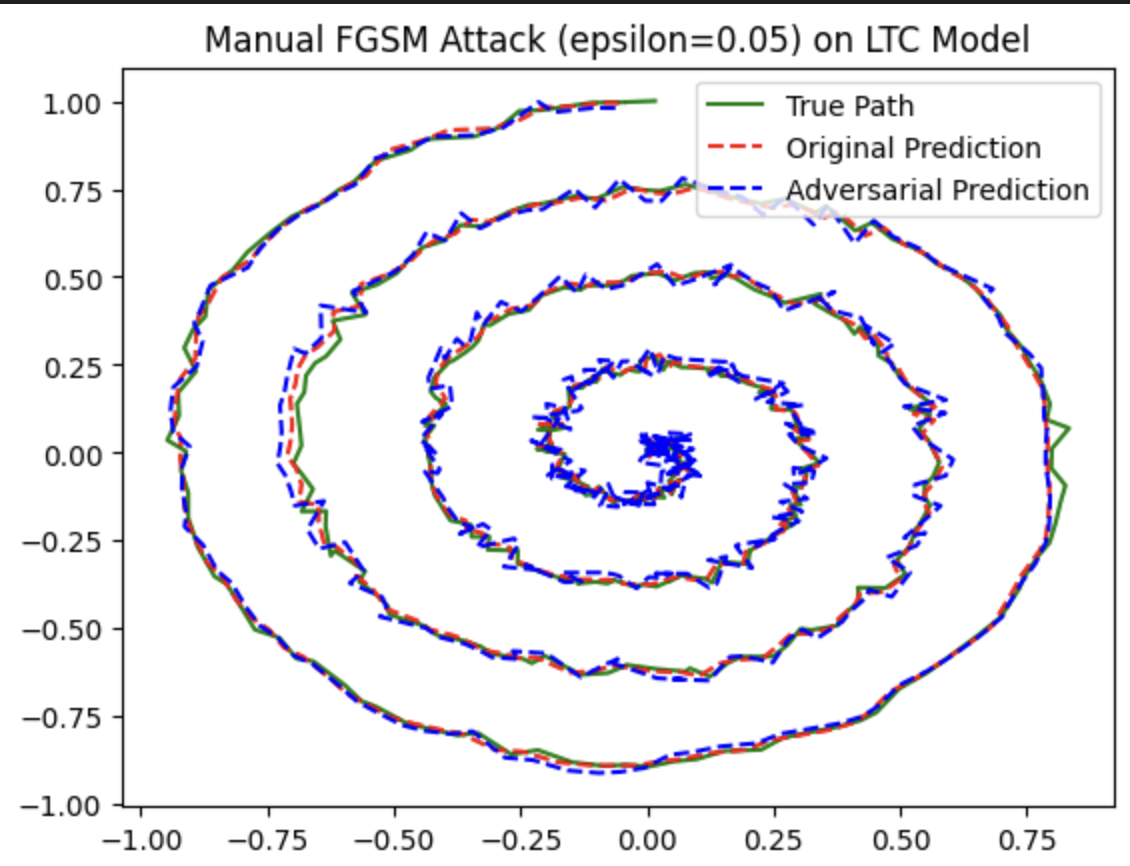
\includegraphics[width=\linewidth]{img/fgsm_spiral_LTC.png}
        \label{fig:fgsm_spiral_LTC}
    \end{subfigure}
    \hfill
    \begin{subfigure}[b]{0.45\linewidth}
        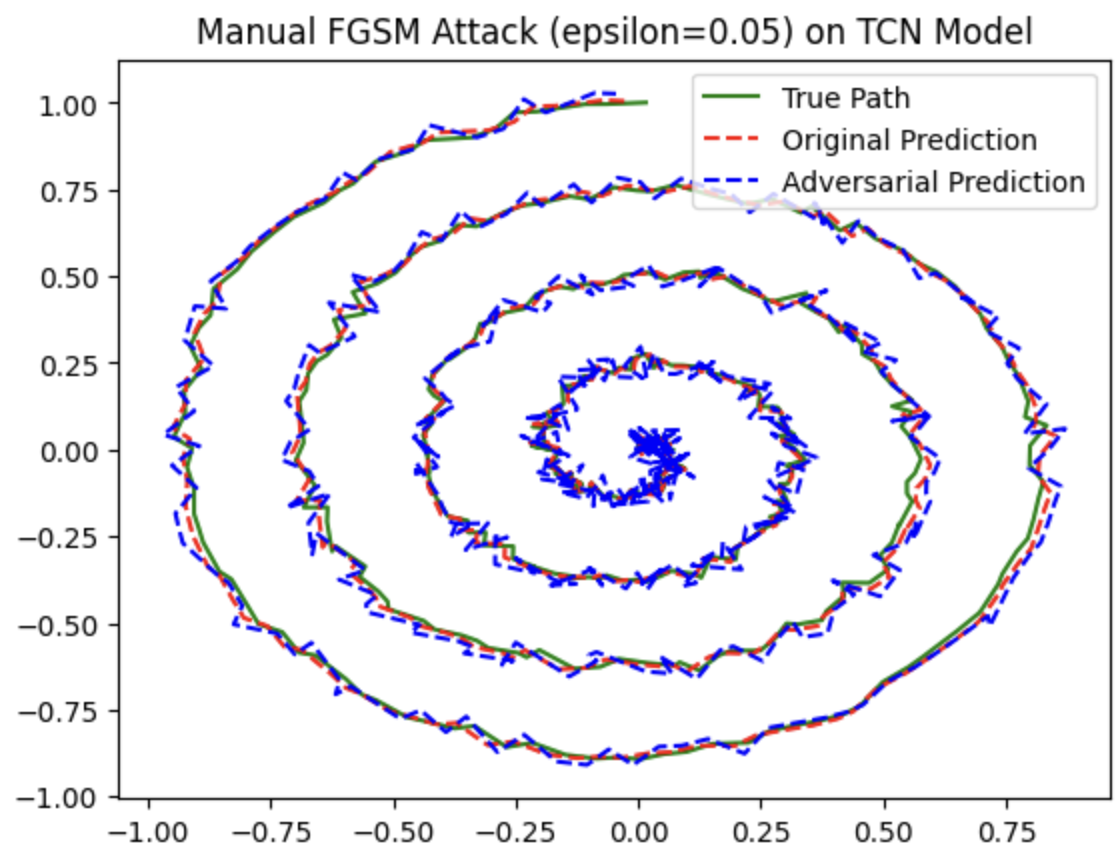
\includegraphics[width=\linewidth]{img/fgsm_spiral_TCN.png}
        \label{fig:fgsm_spiral_TCN}
    \end{subfigure}
    \vskip\baselineskip
    \begin{subfigure}[b]{0.45\linewidth}
        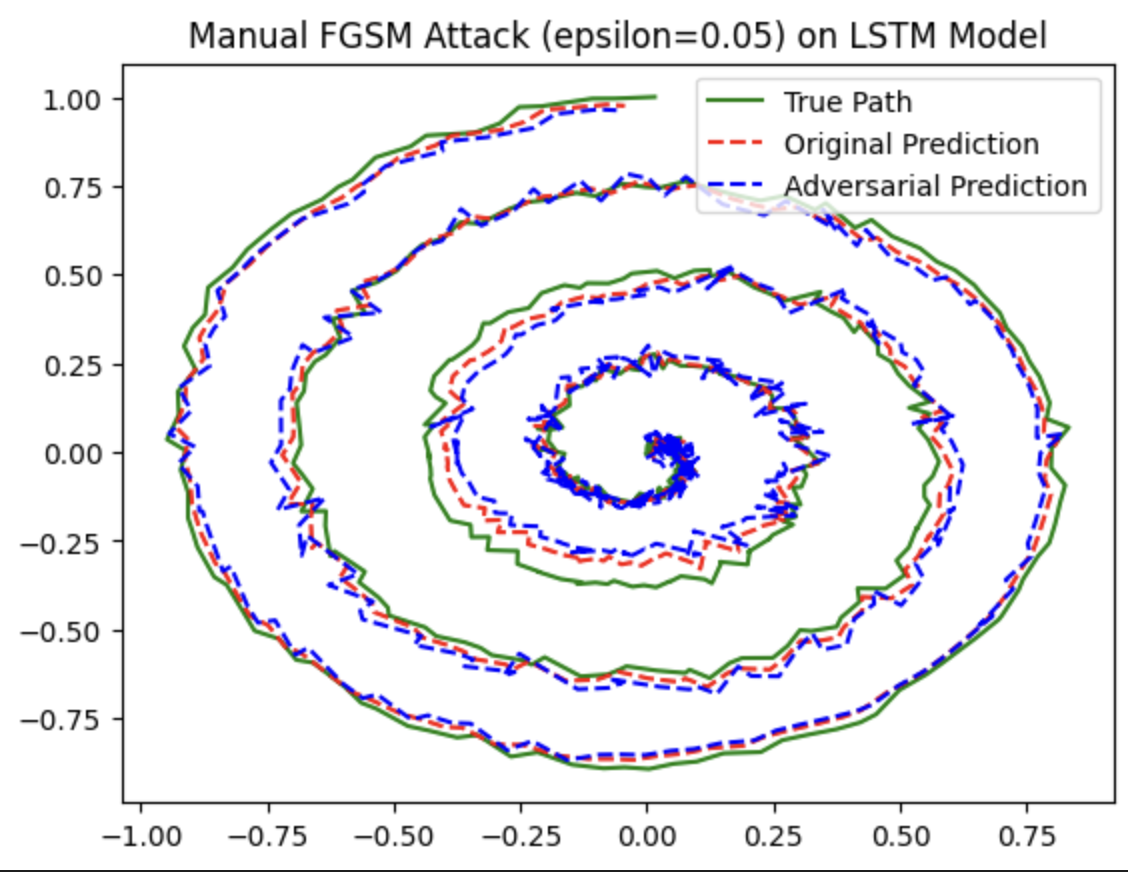
\includegraphics[width=\linewidth]{img/fgsm_spiral_lstm.png}
        \label{fig:fgsm_spiral_lstm}
    \end{subfigure}
    \hfill
    \begin{subfigure}[b]{0.45\linewidth}
        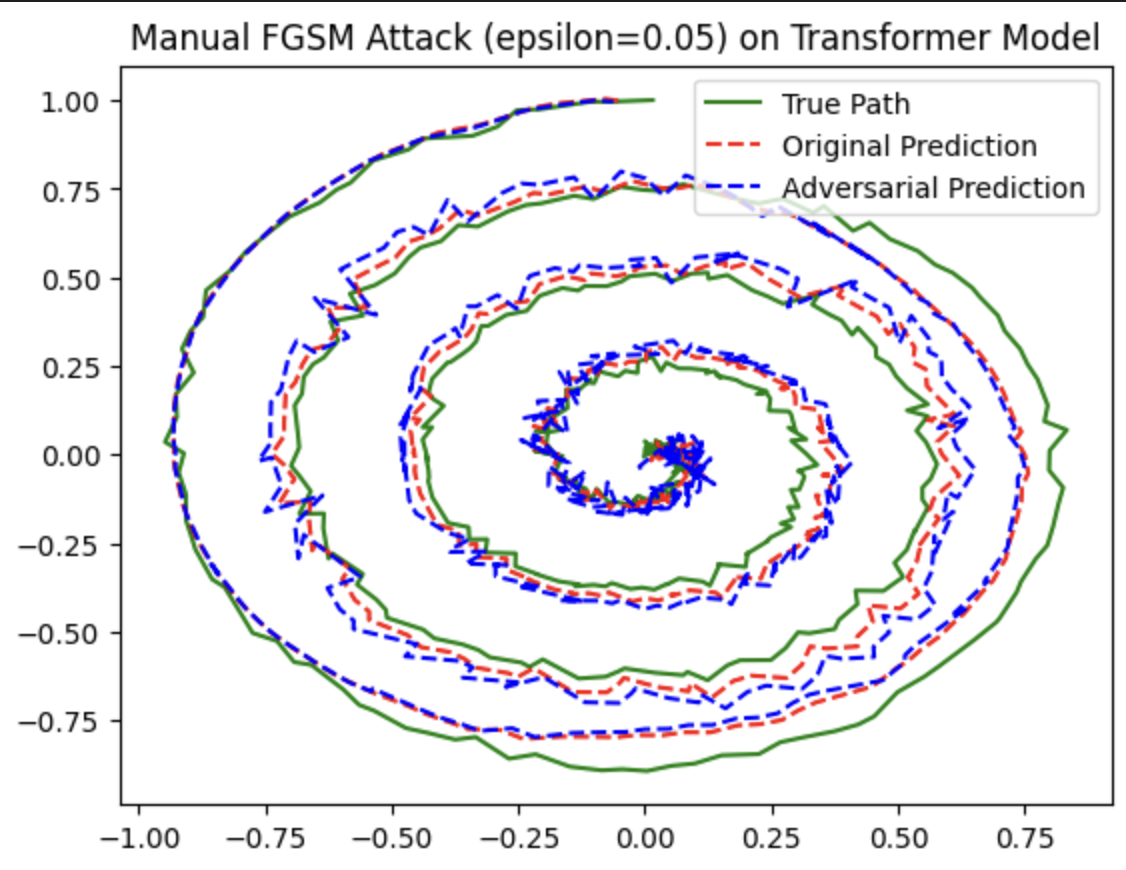
\includegraphics[width=\linewidth]{img/fgsm_spiral_transformer.png}
        \label{fig:fgsm_spiral_transformer}
    \end{subfigure}
    \caption{Predicted, Target, and Adversarial projections under FGSM attack on LTC, TCN, LSTM and Transformer models. Using the same denormalised input spiral.}
    \label{fig:fsgm_spirals}
\end{figure}

From figure~\ref{fig:fsgm_spirals}, the Liquid Neural Network (LTC) shows notable resilience, maintaining close alignment between its original and adversarial predictions for the majority of the trajectory. While minor deviations are visible, especially near the inner spiral, the global structure remains coherent. This is likely due to the continuous-time membrane integration and temporal smoothing induced by the ODE solver.

In contrast, the TCN and Transformer models show pronounced adversarial distortion. The TCN suffers from its lack of recurrent memory, leading to sharp deflections in regions of local perturbation.

The Transformer, despite its capacity, exhibits highly unstable predictions under attack, likely due to its limited inductive bias and sensitivity to global input shifts.

The LSTM model shows intermediate robustness: although its gating structure filters out some perturbations, it remains vulnerable to gradient-based attacks that propagate through long-term memory.

Thus, the LTC's continuous dynamics and biophysical parameterisation seem to have stabilising effect, outperforming the more discrete or attention-based baselines under single-step adversarial pressure.

\subsection*{PGD Attack Results}

PGD, as a stronger attack method, caused greater degradation than FGSM across all models, with stronger effect on deeper temporal structures.

\begin{figure}[H]
    \centering
    \begin{subfigure}[b]{0.45\linewidth}
        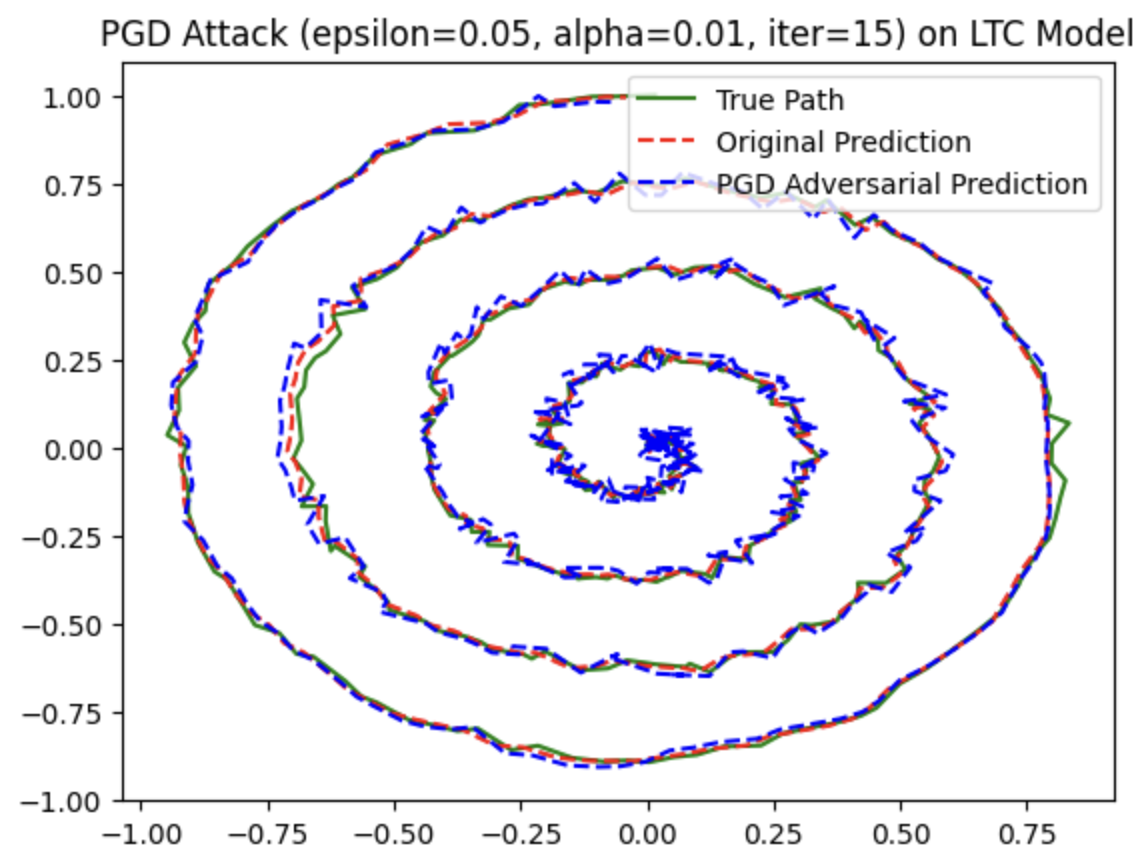
\includegraphics[width=\linewidth]{img/pgd_spiral_LTC.png}
        \label{fig:pgd_spiral_LTC}
    \end{subfigure}
    \hfill
    \begin{subfigure}[b]{0.45\linewidth}
        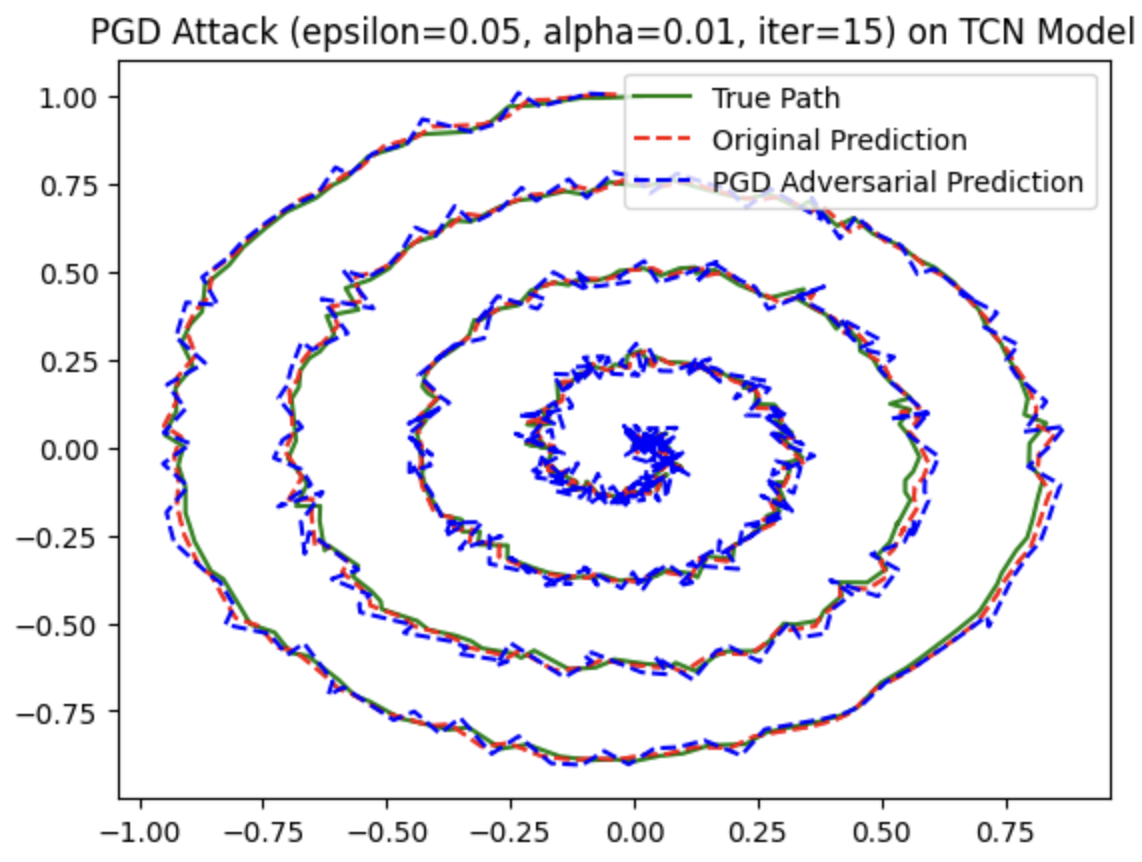
\includegraphics[width=\linewidth]{img/pgd_spiral_TCN.png}
        \label{fig:pgd_spiral_TCN}
    \end{subfigure}
    \vskip\baselineskip
    \begin{subfigure}[b]{0.45\linewidth}
        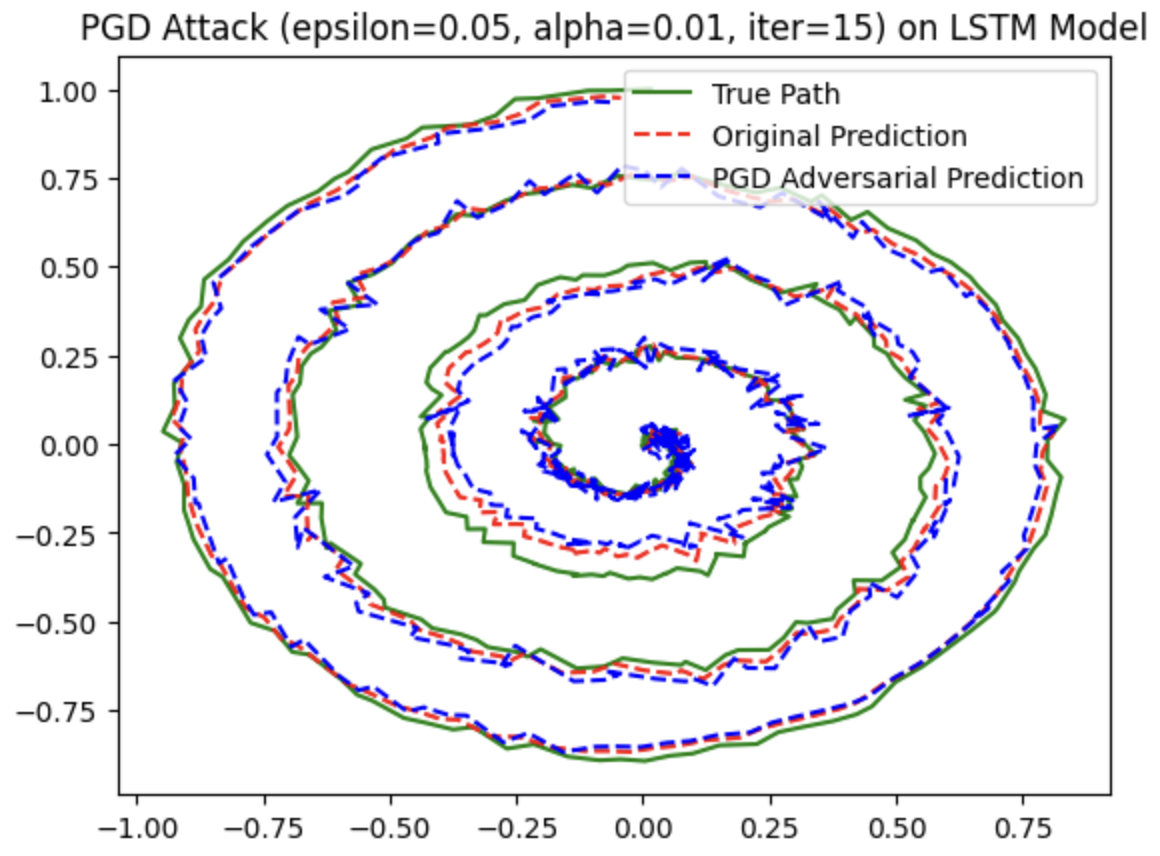
\includegraphics[width=\linewidth]{img/pgd_spiral_lstm.png}
        \label{fig:pgd_spiral_lstm}
    \end{subfigure}
    \hfill
    \begin{subfigure}[b]{0.45\linewidth}
        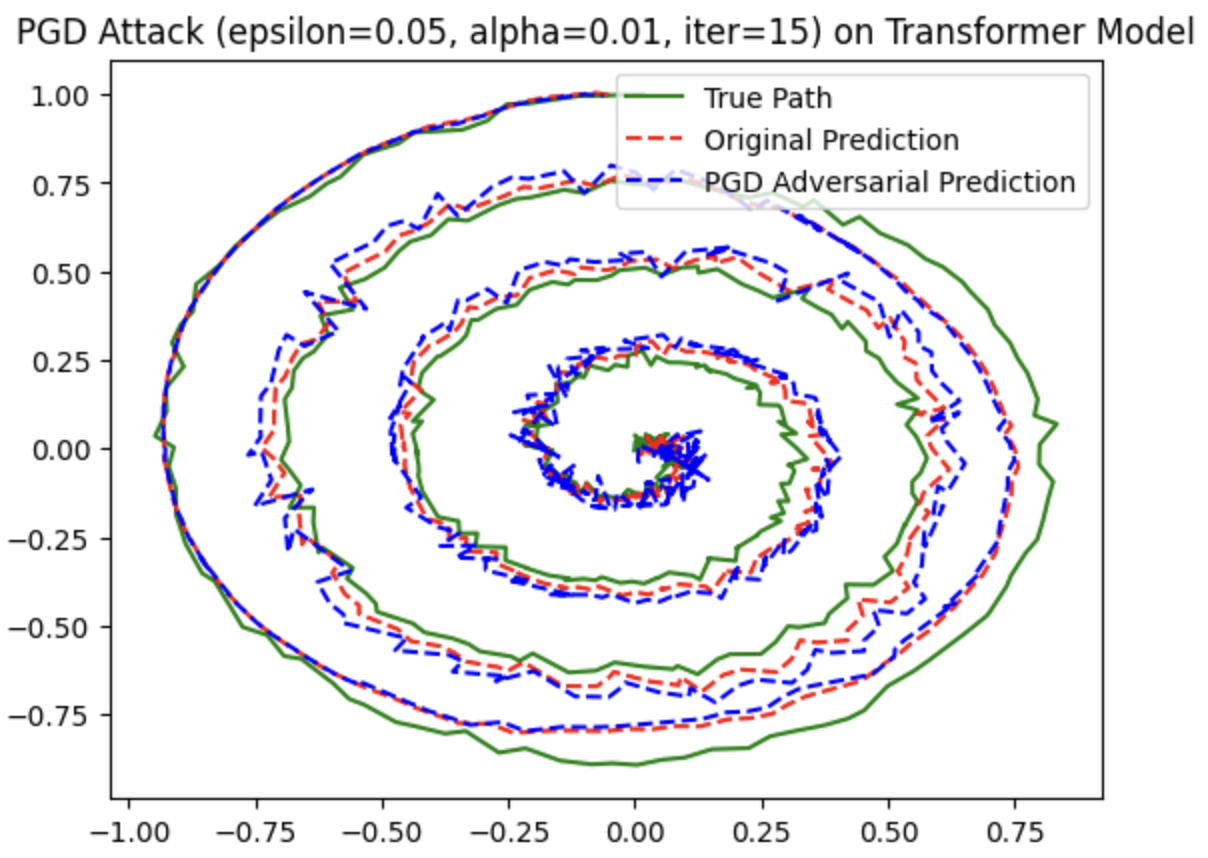
\includegraphics[width=\linewidth]{img/pgd_spiral_transformer.png}
        \label{fig:pgd_spiral_transformer}
    \end{subfigure}
    \caption{Predicted, Target, and Adversarial projections under PGD attack on LTC, TCN, LSTM and Transformer models. Using the same denormalised input spiral.}
    \label{fig:pgd_spirals}
\end{figure}

Figure~\ref{fig:pgd_spirals} presents the effect of a 15-step PGD attack on each model, using $\epsilon = 0.05$ and $\alpha = 0.01$. The LTC continues to exhibit strong robustness, with its adversarial trajectory (blue) closely shadowing the original prediction (red) and the true path (green). Despite minor divergence being visible (particularly near the spiral's centre where curvature is high) the global structure remains largely preserved. This resilience is again due to the regularising effect of continuous-time dynamics and the internal ODE solver. For the PGD attack, this limits perturbations across integration steps, dampening the cumulative effect.

In contrast, the Transformer model suffers substantial degradation. Its adversarial trajectory spirals off course significantly, as a result of the model's sensitivity to small input shifts and lack of temporal inductive bias.

The LSTM also displays clear distortion, particularly in early spiral turns, reflecting how perturbations to the input cascade through long-range memory states. 

The TCN, while affected, shows slightly improved robustness relative to the Transformer and LSTM, likely due to the inherent smoothing effect of its dilated convolutions. The absence of state memory however limits its ability to resist cumulative perturbation.

The LTC model still seems to stabilise stabilise predictions under iterative, gradient-based adversaries like PGD.

\subsection*{Deepfool-Like Attack Results}

\begin{figure}[H]
    \centering
    \begin{subfigure}[b]{0.45\linewidth}
        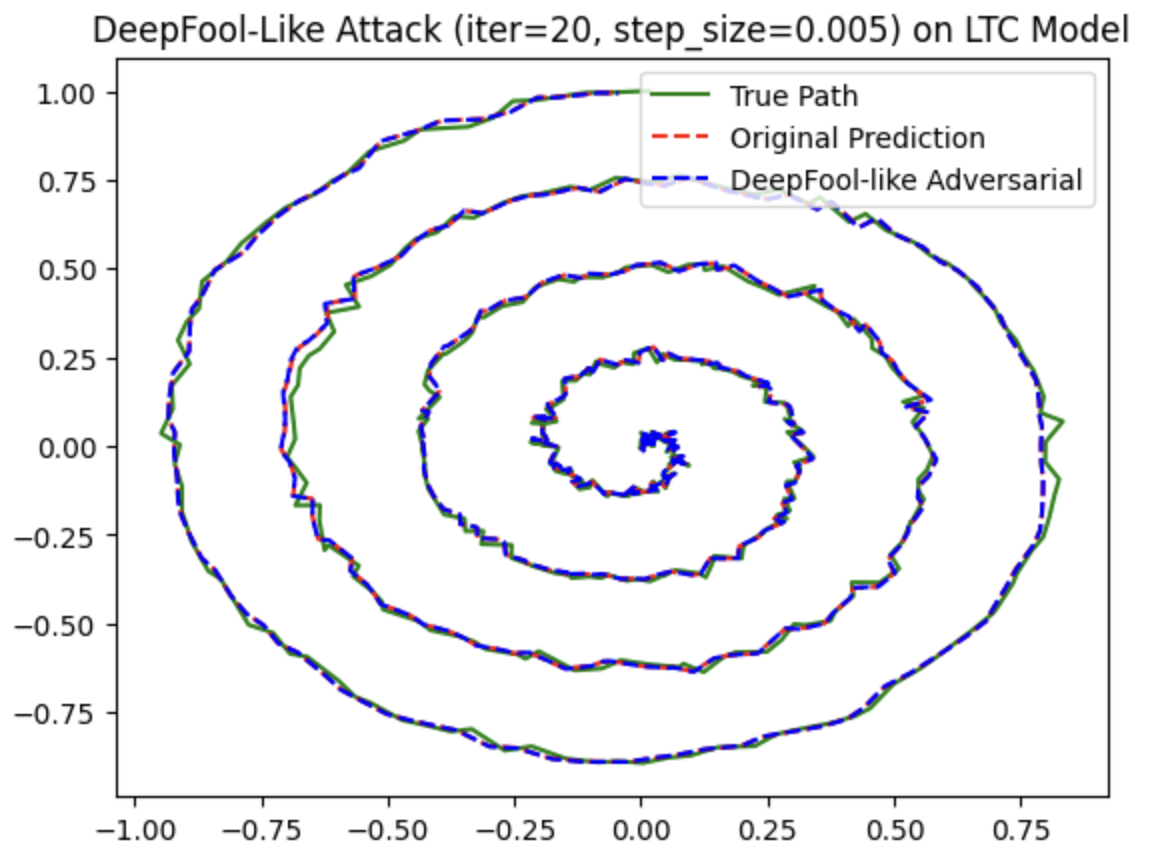
\includegraphics[width=\linewidth]{img/deepfool_spiral_LTC.png}
        \label{fig:deepfool_spiral_LTC}
    \end{subfigure}
    \hfill
    \begin{subfigure}[b]{0.45\linewidth}
        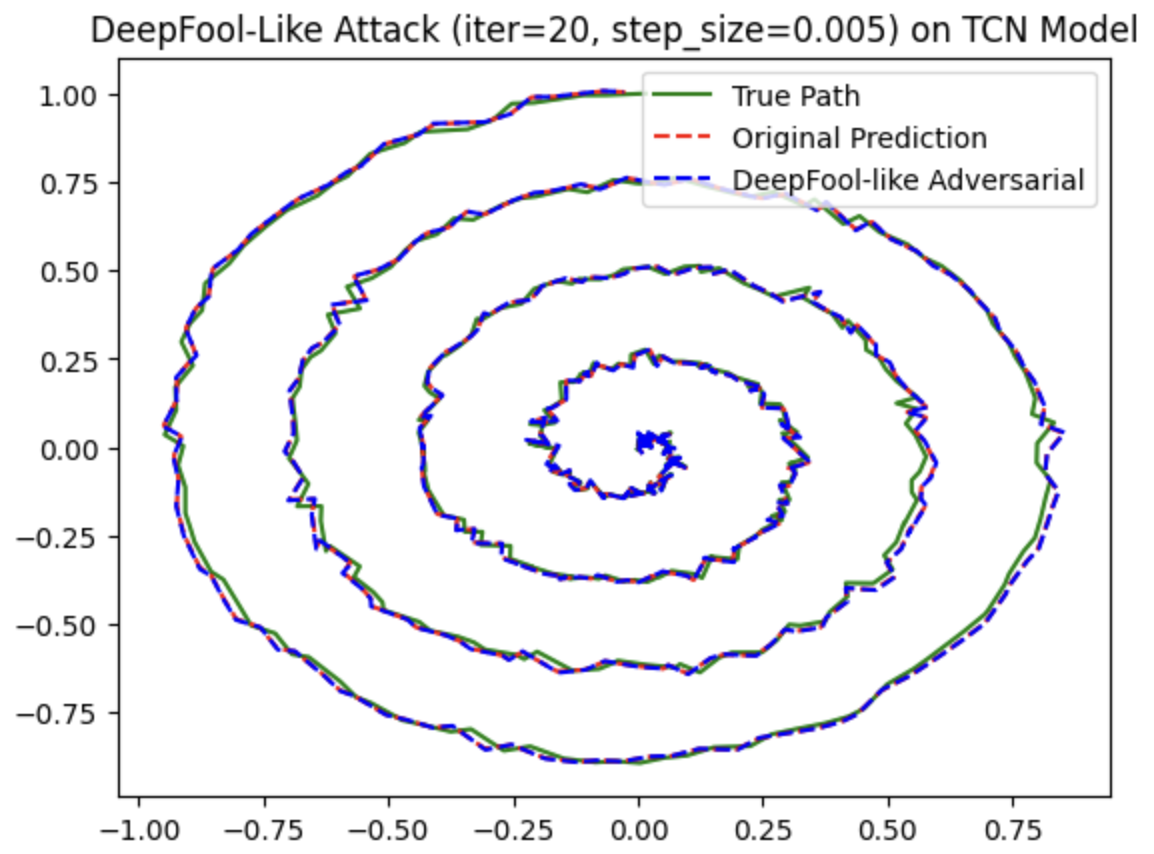
\includegraphics[width=\linewidth]{img/deepfool_spiral_TCN.png}
        \label{fig:deepfool_spiral_TCN}
    \end{subfigure}
    \vskip\baselineskip
    \begin{subfigure}[b]{0.45\linewidth}
        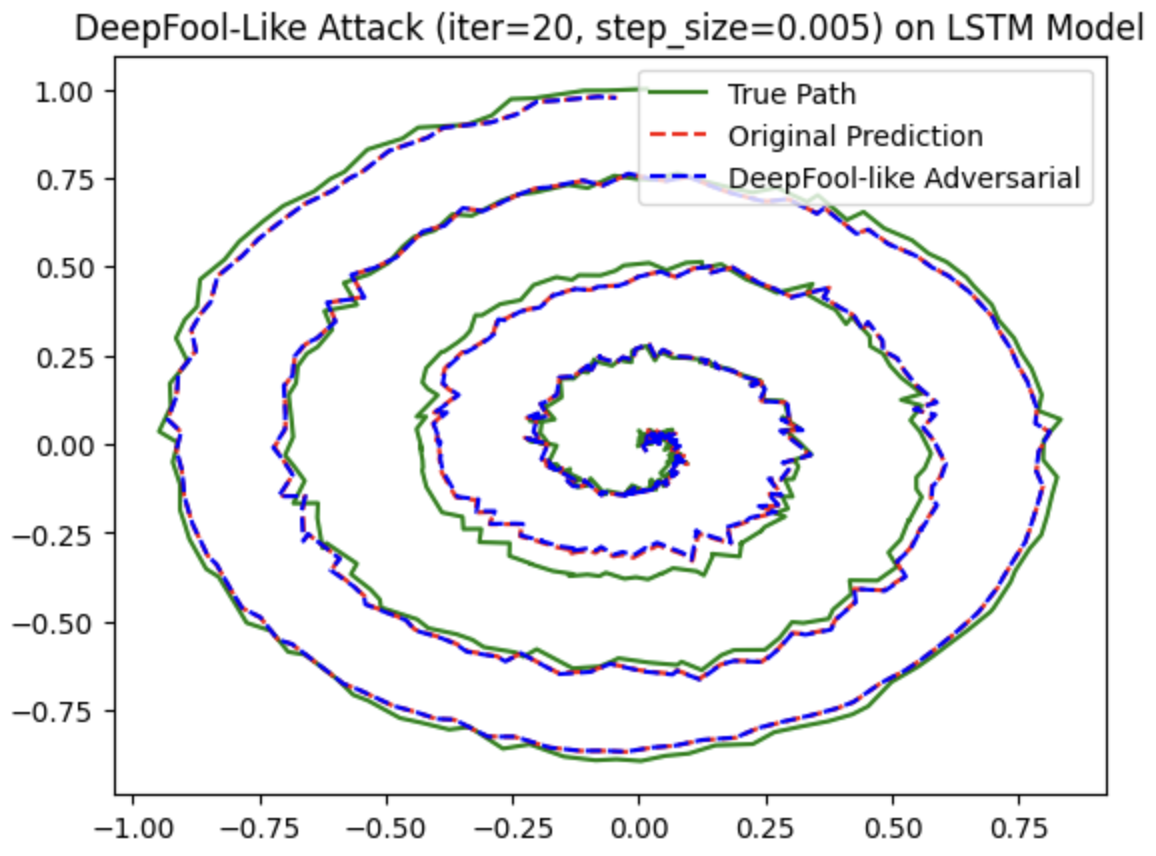
\includegraphics[width=\linewidth]{img/deepfool_spiral_lstm.png}
        \label{fig:deepfool_spiral_lstm}
    \end{subfigure}
    \hfill
    \begin{subfigure}[b]{0.45\linewidth}
        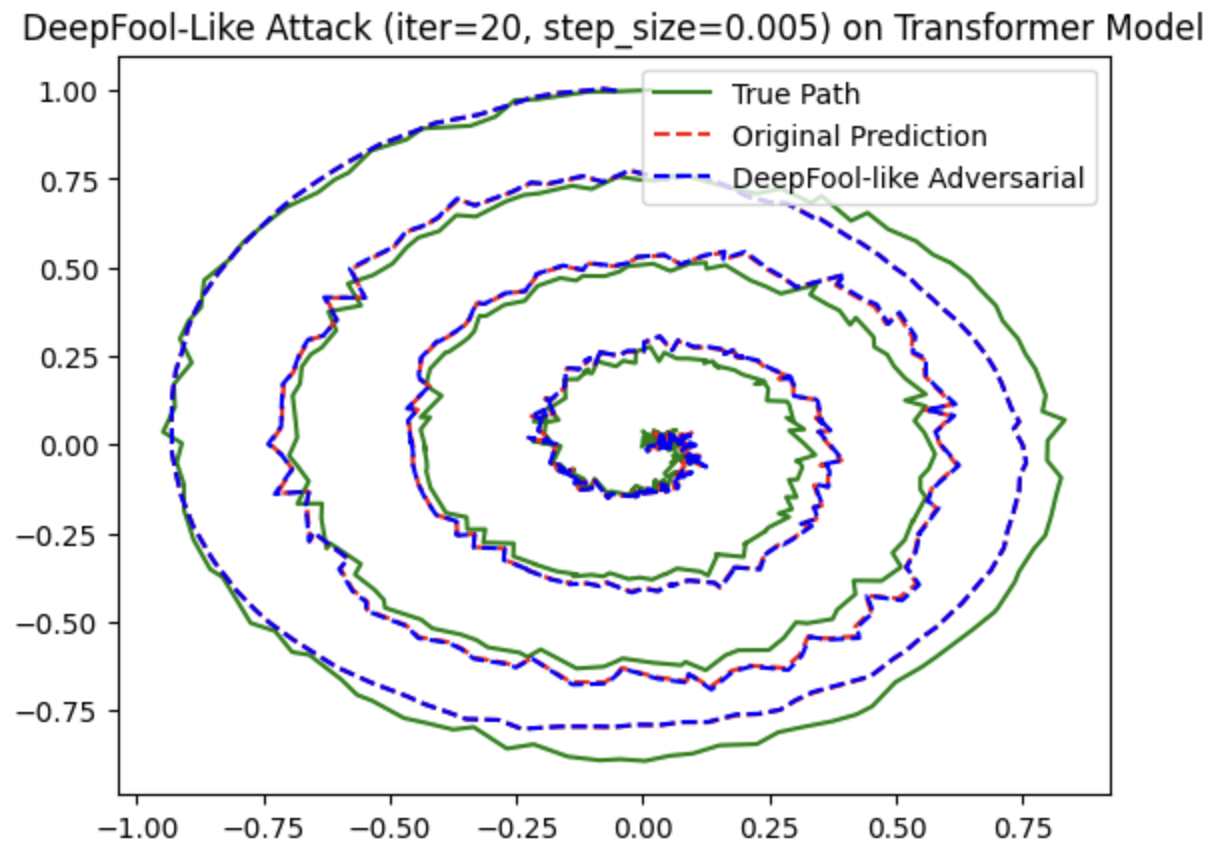
\includegraphics[width=\linewidth]{img/deepfool_spiral_transformer.png}
        \label{fig:deepfool_spiral_transformer}
    \end{subfigure}
    \caption{Predicted, Target, and Adversarial projections under Deepfool-Like attack on LTC, TCN, LSTM and Transformer models. Using the same denormalised input spiral.}
    \label{fig:deepfool_spirals}
\end{figure}

The plots in Figure~\ref{fig:deepfool_spirals} show the effects of a DeepFool-like iterative attack (20 steps, step size = 0.005) adapted for regression. Unlike PGD or FGSM, which aim for maximal distortion within a norm-bound, DeepFool attempts to perturb inputs just enough to cross decision boundaries. In this case, this corresponds to inducing maximal deviation in continuous predictions. The Transformer model shows the highest vulnerability: its adversarial trajectory (blue) diverges significantly from the true path (green), especially in the inner spiral turns where minor distortions amplify rapidly.

The LSTM is similarly affected, to a slightly lesser extent, with perturbations distorting predictions in both early and late sequence segments. This aligns with known vulnerability of memory-based architectures to accumulated gradient signals across time.

The TCN demonstrates moderate resilience. While some deviations occur, especially near tight curvatures, the global shape is retained.

The LTC model remains the most stable under this attack. Its adversarial predictions are closer to the original (red), indicating that the internal ODE dynamics of the LNN may diffuse perturbations temporally, flattening adversarial gradients.

\subsection*{SPSA Results}

\begin{figure}[H]
    \centering
    \begin{subfigure}[b]{0.45\linewidth}
        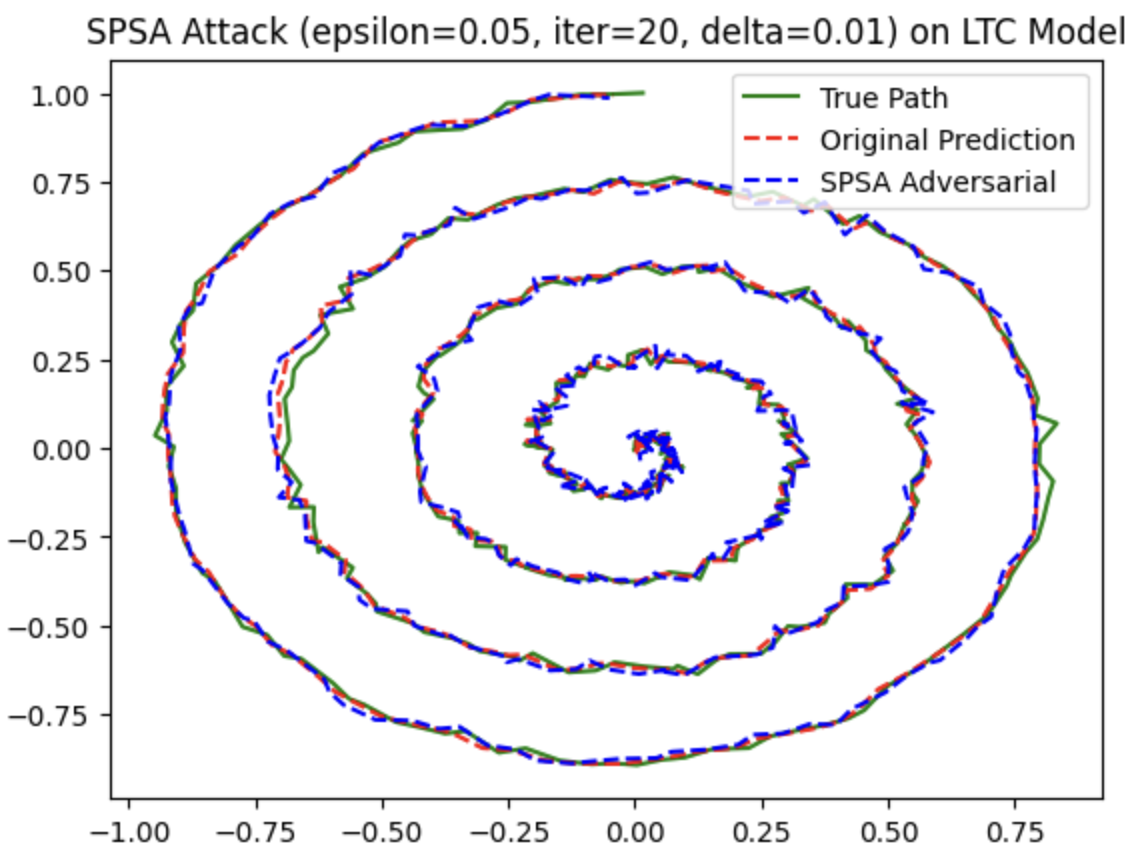
\includegraphics[width=\linewidth]{img/spsa_spiral_LTC.png}
        \label{fig:spsa_spiral_LTC}
    \end{subfigure}
    \hfill
    \begin{subfigure}[b]{0.45\linewidth}
        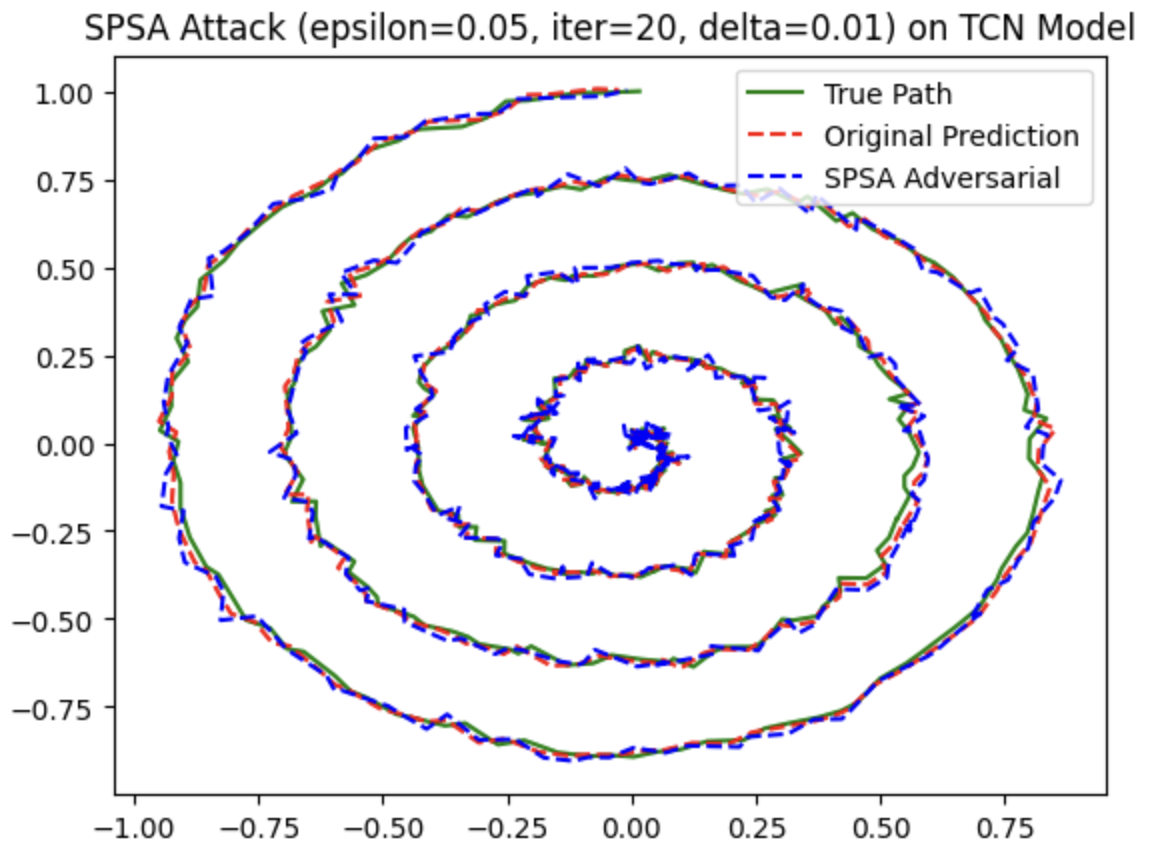
\includegraphics[width=\linewidth]{img/spsa_spiral_TCN.png}
        \label{fig:spsa_spiral_TCN}
    \end{subfigure}
    \vskip\baselineskip
    \begin{subfigure}[b]{0.45\linewidth}
        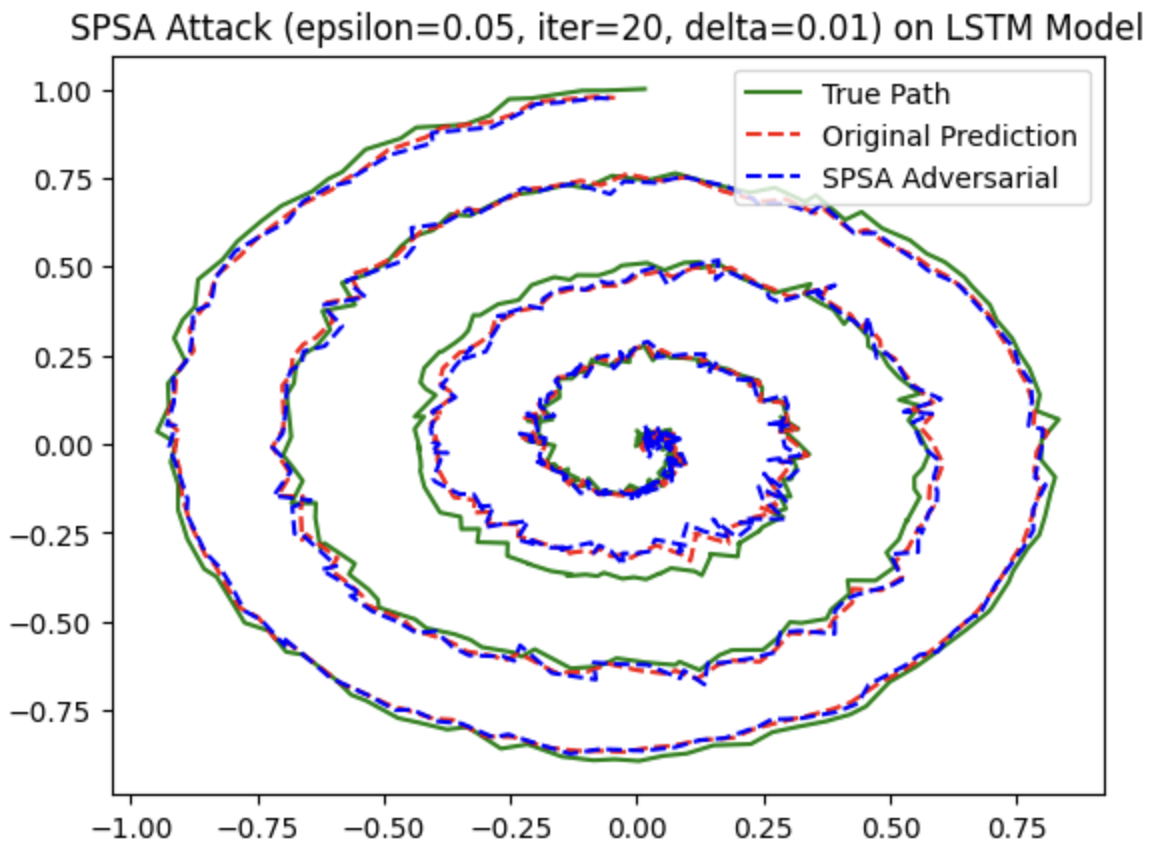
\includegraphics[width=\linewidth]{img/spsa_spiral_lstm.png}
        \label{fig:spsa_spiral_lstm}
    \end{subfigure}
    \hfill
    \begin{subfigure}[b]{0.45\linewidth}
        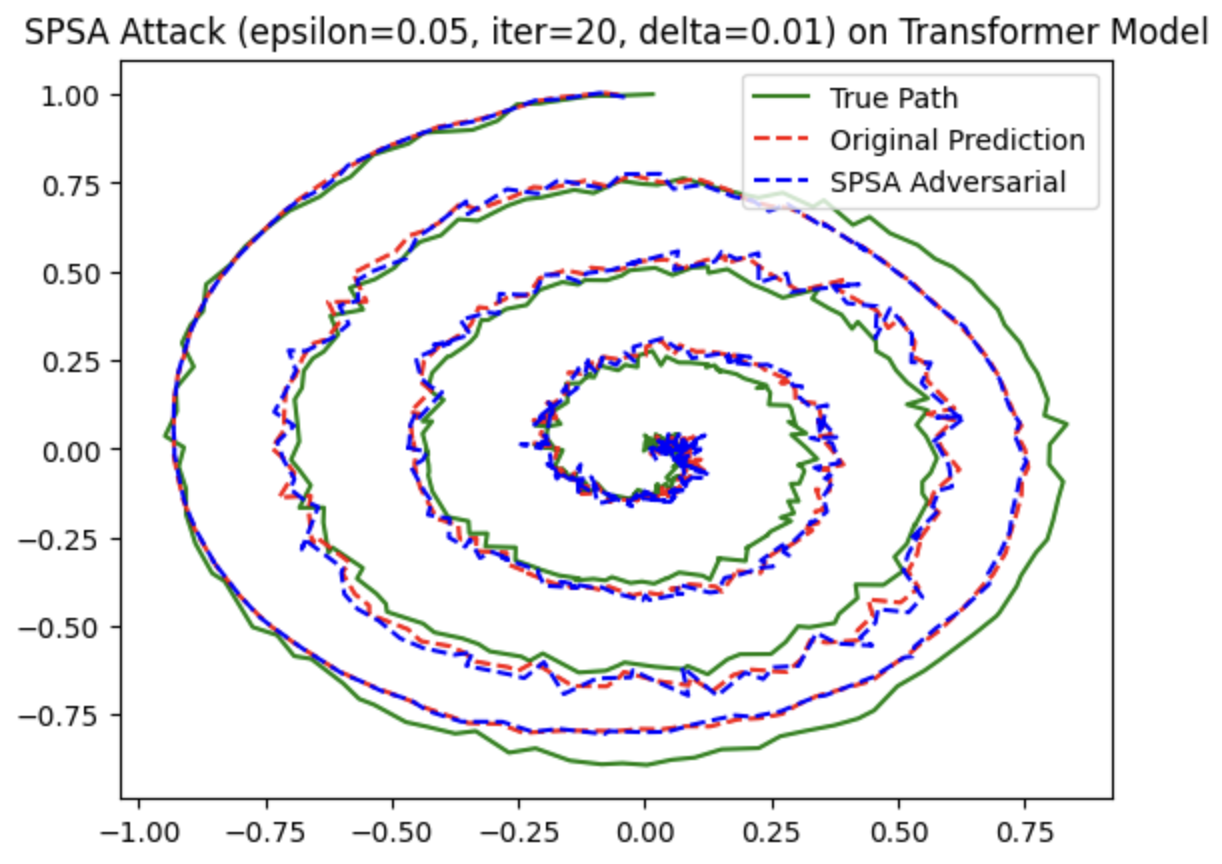
\includegraphics[width=\linewidth]{img/spsa_spiral_transformer.png}
        \label{fig:spsa_spiral_transformer}
    \end{subfigure}
    \caption{Predicted, Target, and Adversarial projections under SPSA attack on LTC, TCN, LSTM and Transformer models. Using the same denormalised input spiral.}
    \label{fig:spsa_spirals}
\end{figure}

As shown in Figure~\ref{fig:spsa_spirals}, the impact of SPSA is comparatively mild across all models, consistent with its tendency to explore less optimal perturbation directions relative to gradient-based attacks like PGD. It does still reveal architectural differences in robustness.

The LTC model shows minimal divergence under SPSA, maintaining tight alignment between original and adversarial predictions. This further reinforces it's resilience observed in prior attack scenarios.

The TCN and Transformer show more visible degradation in the spiral's outer loops, indicating that their fixed receptive fields and positional encoding mechanisms are more easily disrupted by uniform input noise. 

The LSTM shows moderate vulnerability, with adversarial traces deviating steadily from the true trajectory over time.

\subsection*{Time Warping Attack Results}

\begin{figure}[H]
    \centering
    \begin{subfigure}[b]{0.45\linewidth}
        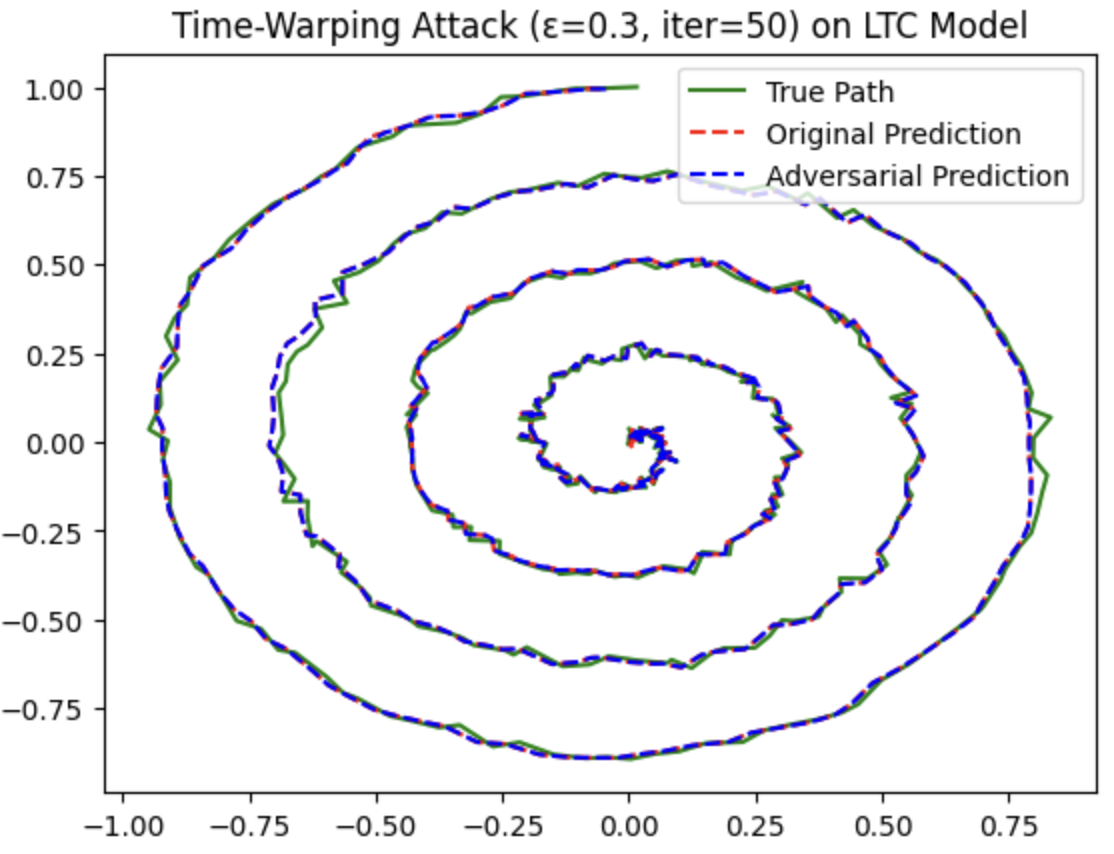
\includegraphics[width=\linewidth]{img/time_warping_spiral_LTC.png}
        \label{fig:time_warping_spiral_LTC}
    \end{subfigure}
    \hfill
    \begin{subfigure}[b]{0.45\linewidth}
        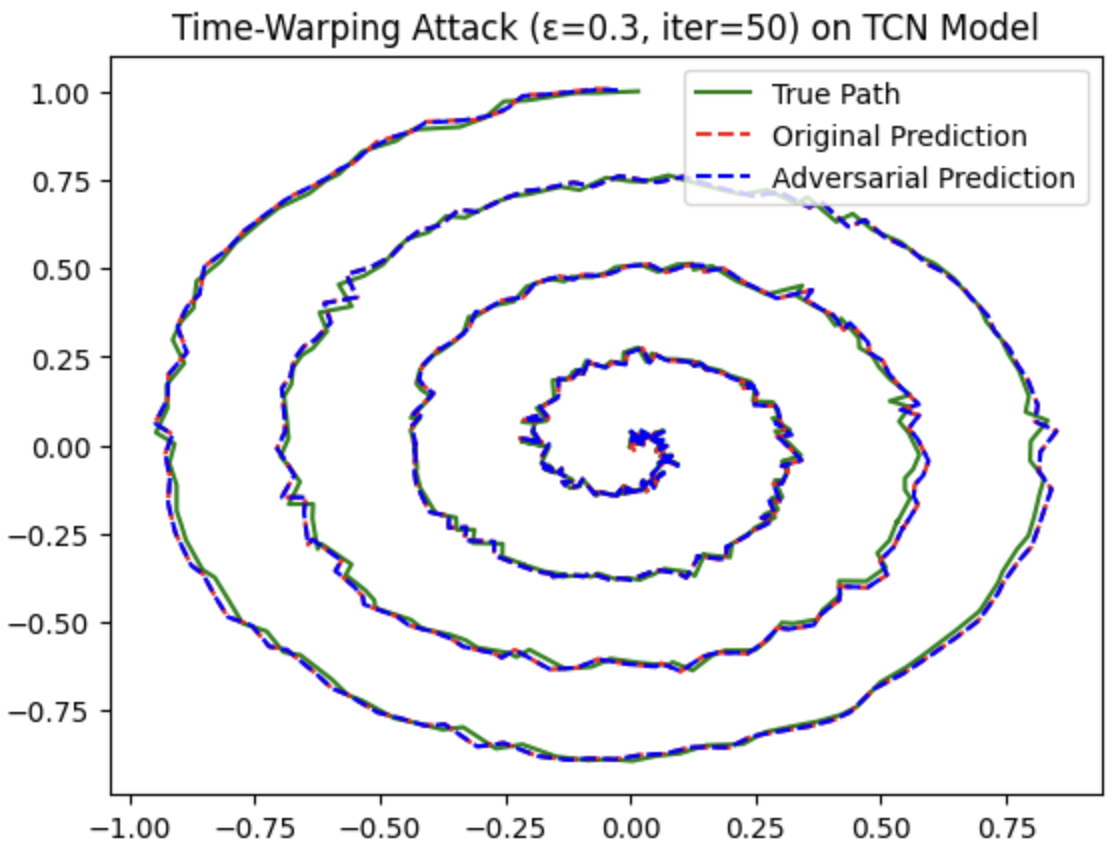
\includegraphics[width=\linewidth]{img/time_warping_spiral_TCN.png}
        \label{fig:time_warping_spiral_TCN}
    \end{subfigure}
    \vskip\baselineskip
    \begin{subfigure}[b]{0.45\linewidth}
        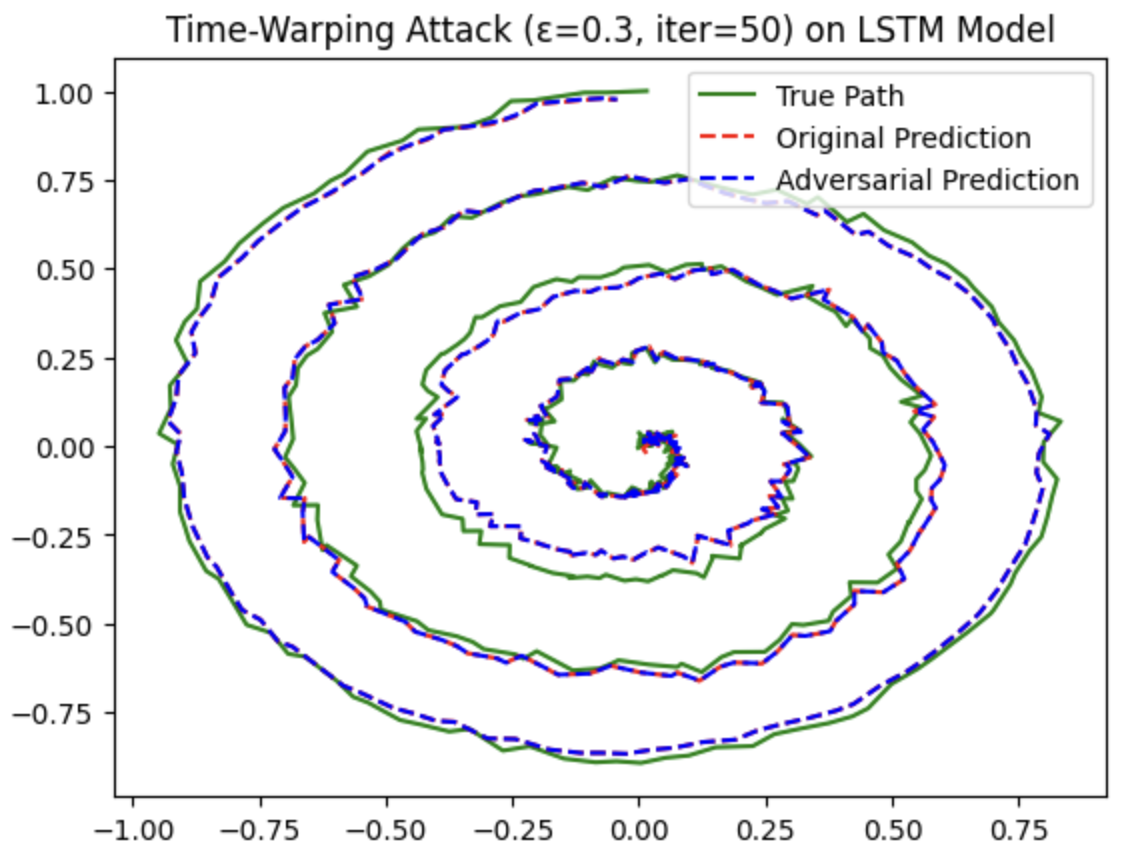
\includegraphics[width=\linewidth]{img/time_warping_spiral_lstm.png}
        \label{fig:time_warping_spiral_lstm}
    \end{subfigure}
    \hfill
    \begin{subfigure}[b]{0.45\linewidth}
        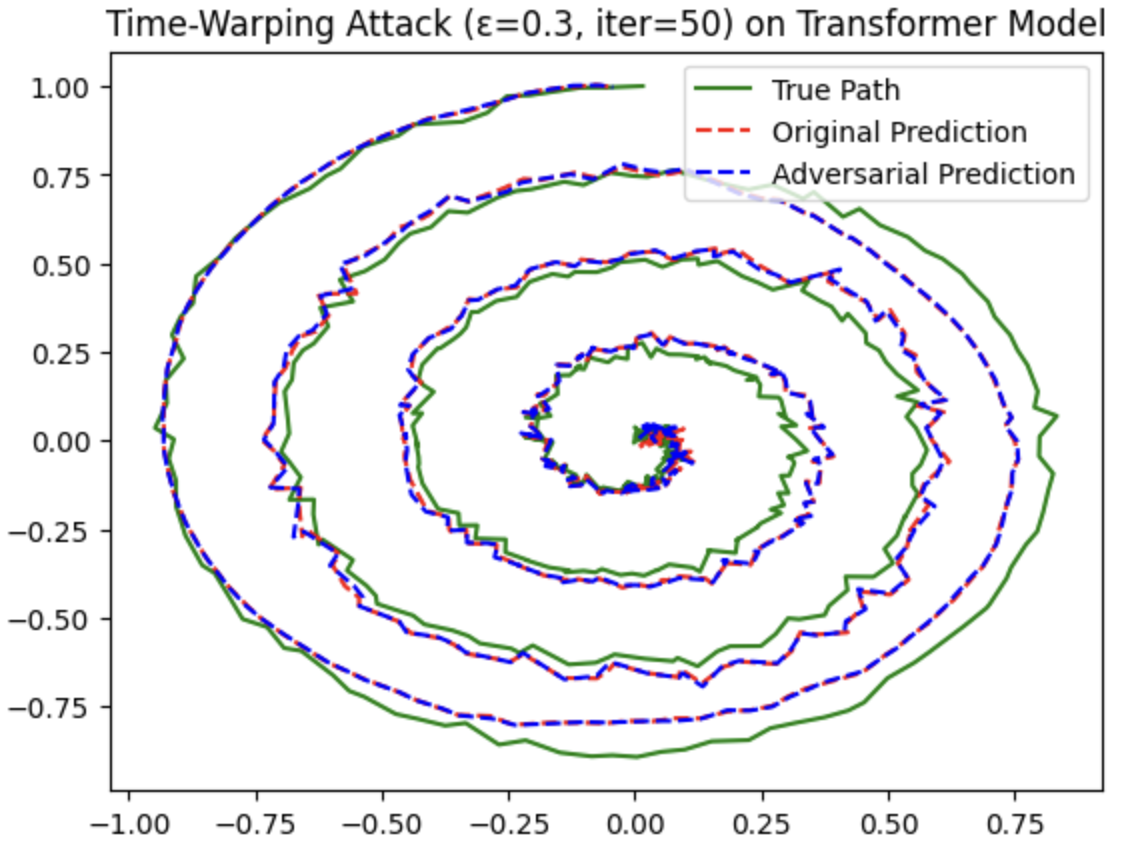
\includegraphics[width=\linewidth]{img/time_warping_spiral_transformer.png}
        \label{fig:time_warping_spiral_transformer}
    \end{subfigure}
    \caption{Predicted, Target, and Adversarial projections under Time Warping attack on LTC, TCN, LSTM and Transformer models. Using the same denormalised input spiral.}
    \label{fig:time_warping_spirals}
\end{figure}

Figure~\ref{fig:time_warping_spirals} displays the impact of a time-warping attack on each model. This attack perturbs the temporal spacing of input points without altering the values themselves, distorting the perceived dynamics of the sequence. The LSTM model appears particularly sensitive, with adversarial predictions deviating noticeably from the true path green, especially in outer spiral turns. This is expected given the LSTM's reliance on a fixed temporal memory structure, which is easily disrupted by misaligned temporal cues.

Similarly, the Transformer struggles to adapt to the warped temporal signal, showing severe prediction drift. This is due to its reliance on position encodings that assume uniform spacing.

In contrast, the TCN maintains good alignment with the true path, showing resilience due to its convolutional structure and dilated receptive fields, which provide a form of local smoothing.

The Liquid Neural Network (LTC) performs best under this attack. Its continuous-time dynamics and internal state integration appear to absorb the warping, maintaining alignment between the adversarial and original predictions. This reinforces the hypothesis that ODE-based temporal models like LNNs are inherently more invariant to temporal distortions, making them better suited for tasks with irregular or corrupted time sampling.

\subsection*{Continuous-Time Adversarial Perturbation Attack Results}

\begin{figure}[H]
    \centering
    \begin{subfigure}[b]{0.45\linewidth}
        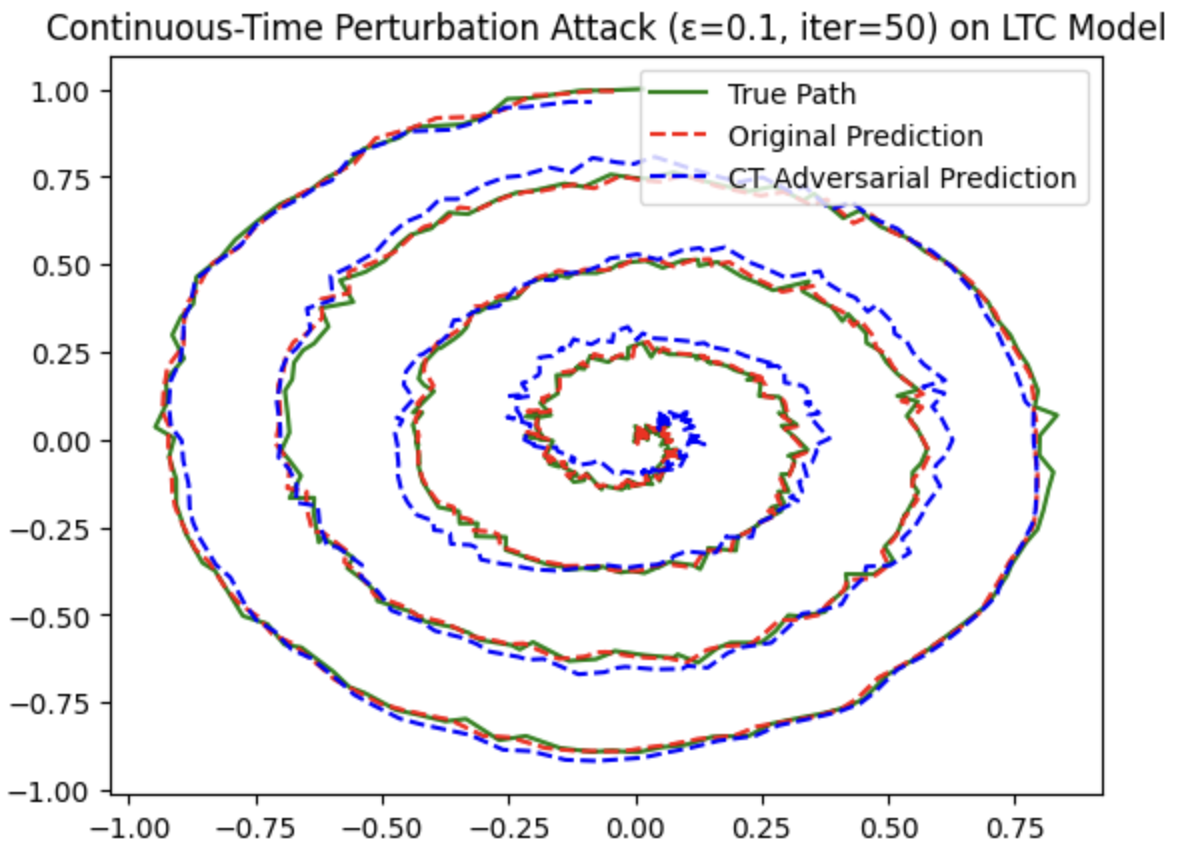
\includegraphics[width=\linewidth]{img/continuous_time_spiral_LTC.png}
        \label{fig:continuous_time_spiral_LTC}
    \end{subfigure}
    \hfill
    \begin{subfigure}[b]{0.45\linewidth}
        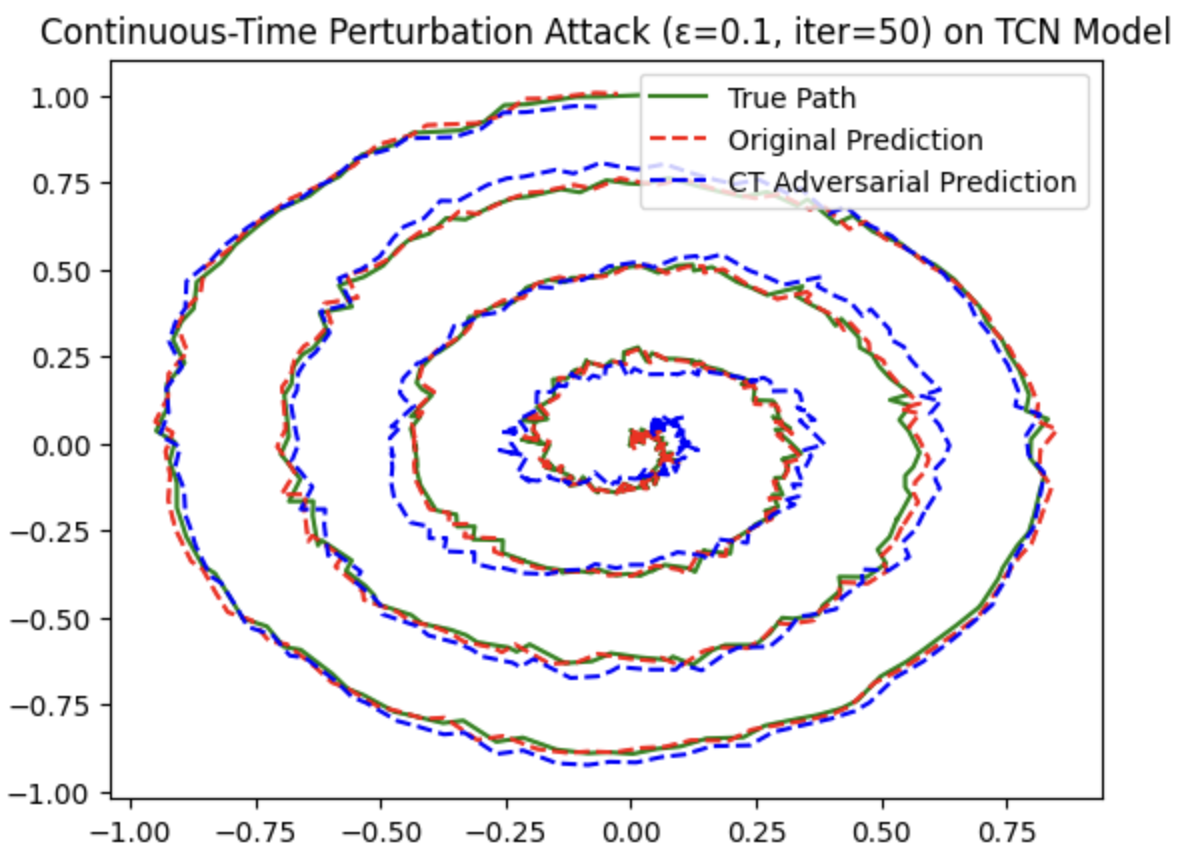
\includegraphics[width=\linewidth]{img/continuous_time_spiral_TCN.png}
        \label{fig:continuous_time_spiral_TCN}
    \end{subfigure}
    \vskip\baselineskip
    \begin{subfigure}[b]{0.45\linewidth}
        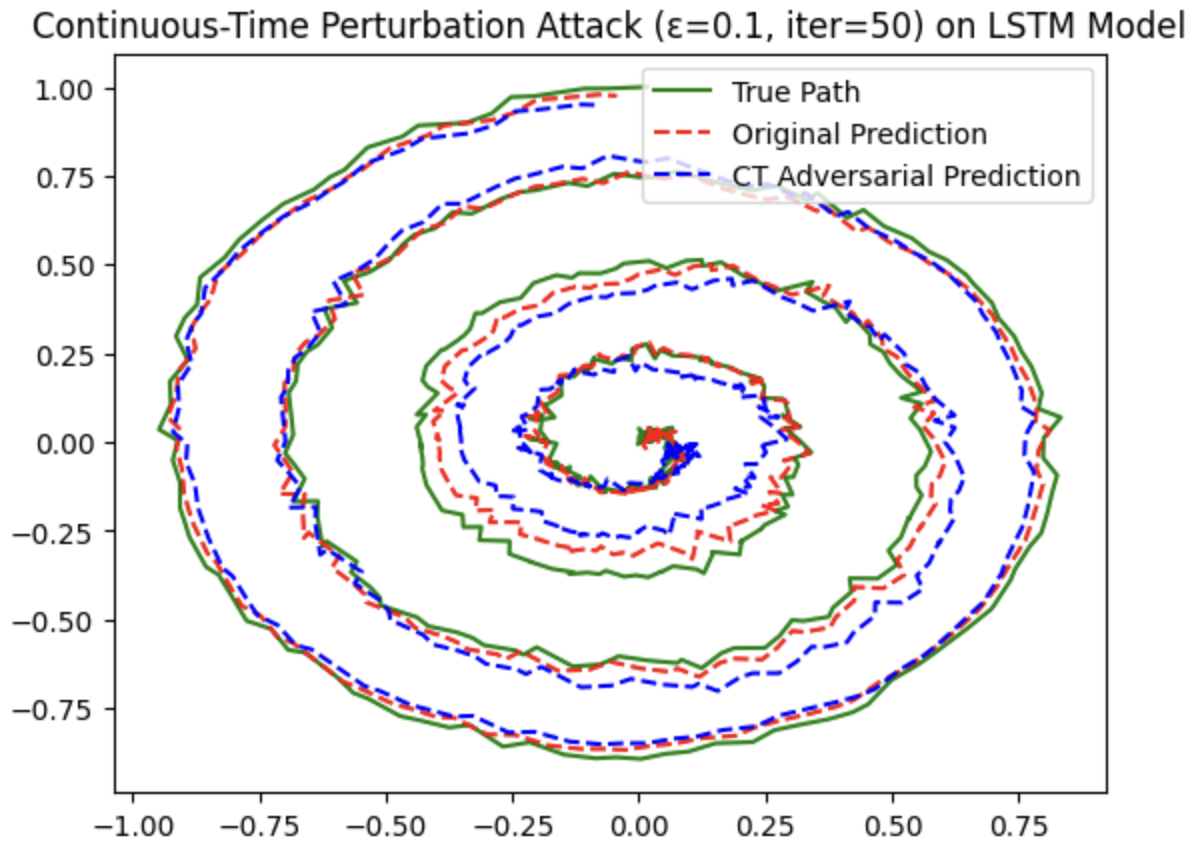
\includegraphics[width=\linewidth]{img/continuous_time_spiral_lstm.png}
        \label{fig:continuous_time_spiral_lstm}
    \end{subfigure}
    \hfill
    \begin{subfigure}[b]{0.45\linewidth}
        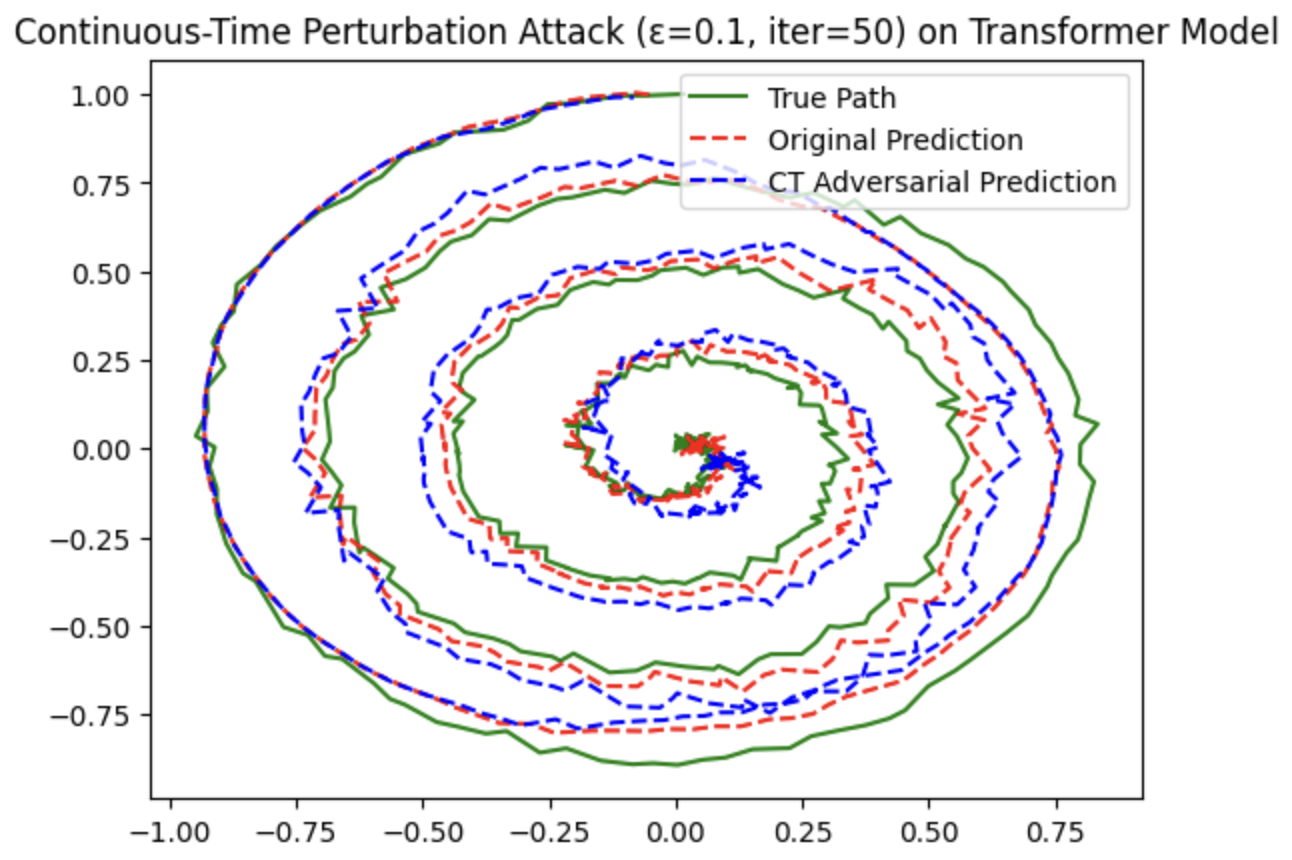
\includegraphics[width=\linewidth]{img/continuous_time_spiral_transformer.png}
        \label{fig:continuous_time_spiral_transformer}
    \end{subfigure}
    \caption{Predicted, Target, and Adversarial projections under Continuous-Time Adversarial Perturbation attack on LTC, TCN, LSTM and Transformer models. Using the same denormalised input spiral.}
    \label{fig:continuous_time_spirals}
\end{figure}

The continuous-time perturbation attack, specifically tailored for models governed by differential equations, targets the latent state evolution rather than directly modifying the input trajectory. This makes it particularly suited for evaluating the Liquid Neural Network (LTC), whose continuous-time membrane dynamics offer both flexibility and potential vulnerability to such perturbations.

As shown in Figure~\ref{fig:continuous_time_spirals}, the LTC model remains relatively stable under attack, with adversarial predictions closely tracking the original predictions throughout the spiral. This indicates that the internal ODE dynamics, when properly regularised, can absorb structured noise and maintain functional predictions.

The TCN and LSTM models however exhibit more pronounced deviations, especially in the outer spiral turns, suggesting that perturbations which indirectly affect temporal relationships (e.g. via integration-like behaviour) are disruptive to their sequential representations.

The Transformer, which lacks an explicit temporal evolution mechanism, is highly vulnerable to these perturbations, with the adversarial trajectory diverging significantly from the true path.

This again highlights a key advantage of biologically inspired continuous-time models (LNNs) in handling dynamic, structured adversarial noise.

\subsection*{Interpretation}

Models with rigid temporal assumptions or recurrent memory (LSTM) are more susceptible to both magnitude and timing distortions, whereas continuous-time dynamics (LNN) offer meaningful resistance. However, no model was universally robust, and each architecture exhibited specific weaknesses when faced with particular perturbation types.

\section{Discussion of Results}

\subsection*{Architecture-Specific Vulnerabilities}

A cross-attack comparison reveals that each model exhibits distinct vulnerabilities determined by its inductive biases. The LSTM is particularly sensitive to early-sequence perturbations due to its recurrent memory, leading to long-range compounding errors. TCNs, while able to contain noise locally, struggle to restore global structure after distortion. The Transformer's self-attention allows some recovery via context redistribution, but it remains susceptible to phase collapse under structured attacks (when key tokens are disrupted). The Liquid Neural Network (LNN), by contrast, preserves smoothness but responds poorly to high-frequency or temporally persistent adversaries, as shown in its high degradation under continuous-time and PGD perturbations.

\subsection*{Model Design}

These results align with the models' architectural design. LSTMs encode state recursively, which amplifies small errors. TCNs filter over fixed windows, making them blind to long-term disruptions. Transformers rely on positional encoding without state memory, making them sensitive to ordering distortions. LNNs model time explicitly via ODEs, offering natural resistance to time-warping and continuity-based attacks, but remain dependent on solver stability and hyperparameter tuning.

\subsection*{Temporal Drift and Geometric Collapse}

A consistent phenomenon observed in PGD, DeepFool-like, and continuous-time attacks is phase drift. This is where adversarial trajectories spiral inward or outward over time. This error accumulates directionally rather than randomly, reflecting the effectiveness of gradient-aligned perturbations in destabilising long-term dynamics.

Attacks like FGSM and SPSA however result in less coherent but more transient distortions, typically recoverable unless they coincide with critical points in the trajectory.

\section{Defences for Liquid Neural Networks}

There are a range of theoretical strategies that can be used to mitigate adversarial vulnerability in Liquid Neural Networks (LNNs), with comparisons to TCN and LSTM where relevant.

\subsection*{Adversarial Training and Perturbation Smoothing}

While adversarial training has been shown effective in conventional networks \cite{madry2018towards}, its adaptation to continuous-time models like LNNs requires careful consideration. One potential direction is continuous-time adversarial training, where adversarial perturbations are applied not only at the input level but across intermediate ODE solver steps. This would simulate realistic, dynamic threats such as time-warping or sensor noise.

In addition, input noise injection (e.g. Gaussian or uniform noise) could promote smoother input-output mappings, as seen in denoising autoencoders \cite{vincent2008extracting}. For LNNs, perturbing the input current $u_i(t)$ over time can improve resistance to minor temporal distortions.

\subsection*{Structural Regularisation in Liquid Architectures}

A core advantage of LNNs lies in their biologically-inspired dynamics:
\begin{equation}
\frac{dv_i}{dt} = -\frac{v_i}{\tau} + \sum_j W_{ij} \cdot \sigma(v_j(t)) + u_i(t)
\end{equation}

Here, the decay constant $\tau$ and activation function $\sigma$ are learnable. Imposing soft constraints on $\tau$ or bounding the membrane potential $v_i$ could prevent exponential state divergence under perturbation.

\textbf{Figure~\ref{fig:lnn_dynamics_defence}} illustrates how limiting the slope of the state curve over time may preserve stability.

\begin{figure}[H]
    \centering
    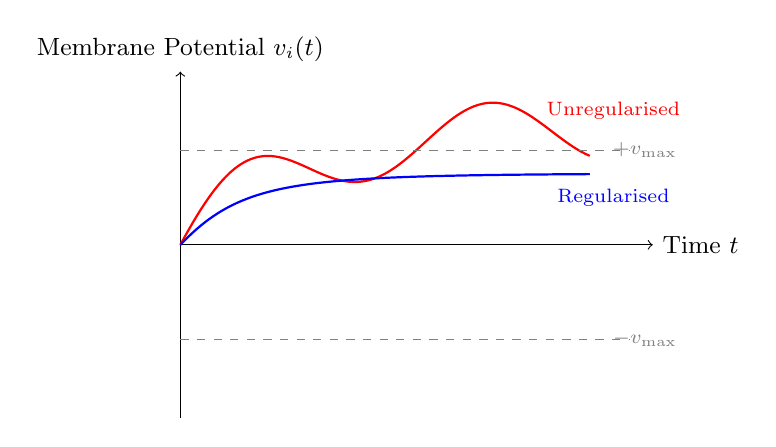
\begin{tikzpicture}[scale=1.0, every node/.style={font=\small}]
        % Axes
        \draw[->] (0,0) -- (6,0) node[right] {Time $t$};
        \draw[->] (0,-2.2) -- (0,2.2) node[above] {Membrane Potential $v_i(t)$};
    
        % Unregularised curve (exponential growth)
        \draw[red, thick, domain=0:5.2, samples=100] plot (\x, {1.5*(1 - exp(-0.7*\x)) + 0.4*sin(2*\x r)});
        \node[red] at (5.5,1.7) {\scriptsize Unregularised};
    
        % Regularised curve (bounded)
        \draw[blue, thick, domain=0:5.2, samples=100] plot (\x, {tanh(1.5*(1 - exp(-0.7*\x)))});
        \node[blue] at (5.5,0.6) {\scriptsize Regularised};
    
        % Horizontal dashed lines (bounds)
        \draw[dashed, gray] (0,1.2) -- (5.7,1.2);
        \draw[dashed, gray] (0,-1.2) -- (5.7,-1.2);
        \node[gray] at (5.9,1.2) {\scriptsize $+v_{\max}$};
        \node[gray] at (5.9,-1.2) {\scriptsize $-v_{\max}$};
    \end{tikzpicture}
    \caption{LNN membrane potential evolution with and without regularisation. Regularisation limits state drift, improving stability under input perturbations.}
    \label{fig:lnn_dynamics_defence}
    \end{figure}

Additionally, dynamically adjusting the solver step size during inference (based on detected input smoothness or gradient norms) can act as another form of defence. Such adaptive schemes are supported by work in neural ODE robustness \cite{dupont2019augmented, finlay2020trainable}.

\subsection*{Temporal Input Filtering and Quantisation}

Preprocessing defences offer architecture-agnostic robustness benefits. Applying a low-pass filter to the input trajectory, defined as:
\begin{equation}
x_t^{\text{filtered}} = \alpha x_t + (1 - \alpha) x_{t-1}, \quad \alpha \in [0, 1]
\end{equation}
can suppress high-frequency adversarial noise typical in gradient-based attacks.

Similarly, discretising the time component or input position encoding:
\begin{equation}
\text{quantised}_t = \left\lfloor \frac{t}{\Delta t} \right\rfloor
\end{equation}
has been hypothesised to improve invariance to small timing shifts \cite{wang2018adversarial}.

% \begin{figure}[H]
% \centering
% \includegraphics[width=0.65\linewidth]{img/temporal_filtering.png}
% \caption{Illustration of low-pass temporal filtering as a defence mechanism. Sharp perturbations are smoothed before reaching the model.}
% \label{fig:temporal_filter}
% \end{figure}

\begin{figure}[H]
    \centering
    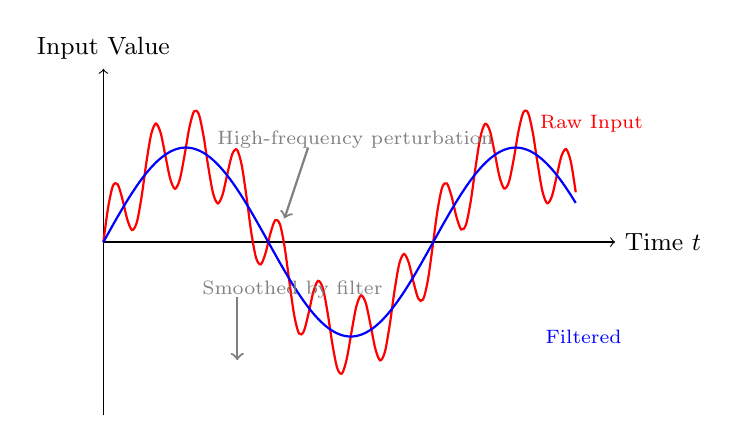
\begin{tikzpicture}[scale=1.0, every node/.style={font=\small}]
        % Axes
        \draw[->] (0,0) -- (6.5,0) node[right] {Time $t$};
        \draw[->] (0,-2.2) -- (0,2.2) node[above] {Input Value};
    
        % Raw input signal (with perturbations)
        \draw[red, thick, domain=0:6, samples=100, smooth] plot (\x, {1.2*sin(1.5*\x r) + 0.5*sin(12*\x r)});
        \node[red] at (6.2,1.5) {\scriptsize Raw Input};
    
        % Filtered signal
        \draw[blue, thick, domain=0:6, samples=100, smooth] plot (\x, {1.2*sin(1.5*\x r)});
        \node[blue] at (6.1,-1.2) {\scriptsize Filtered};
    
        % Noise label
        \draw[->, thick, gray] (2.6,1.2) -- (2.3,0.3);
        \node[gray] at (3.2,1.3) {\scriptsize High-frequency perturbation};
    
        % Filter label
        \draw[->, thick, gray] (1.7,-0.7) -- (1.7,-1.5);
        \node[gray] at (2.4,-0.6) {\scriptsize Smoothed by filter};
    
    \end{tikzpicture}
    \caption{Illustration of low-pass temporal filtering as a defence mechanism. Sharp perturbations are smoothed before reaching the model.}
    \label{fig:temporal_filter}
    \end{figure}

\subsection*{Inductive Bias and Solver-Aware Stability}

Unlike discrete models, LNNs require the solver to faithfully capture non-linear temporal dynamics. This opens unique defence opportunities:
\begin{itemize}
\item \textbf{Step-size modulation:} Smaller solver steps reduce numerical error accumulation under perturbed inputs.
\item \textbf{Activation bounding:} Enforcing $|v_i(t)| \leq V_\text{max}$ could prevent state explosion.
\item \textbf{Implicit regularisation:} Using solver-aware loss terms penalising high curvature over time.
\end{itemize}

These mechanisms can be integrated during training to enforce smooth, stable behaviour even when inputs deviate adversarially.

\subsection*{Limitations}

Liquid models do also present unique challenges, since adversarial attacks in continuous time are underexplored and difficult to formalise. Solver regularisation may reduce model expressivity or increase compute cost. There is also a risk that filtering can remove meaningful signal patterns in real-world tasks.

Practially incorporating formal verification \cite{zhang2022towards} or hybrid models that mix discrete and continuous pathways may further improve LNN reliability.
